\documentclass[12pt]{article}
\usepackage[ukrainian,shorthands=off]{babel}   % shorthands=off: символ " не активний (потрібно для міток "..." у TikZ всередині \zadtask)
\usepackage{fontspec}
% --- НАЛАШТУВАННЯ ШРИФТІВ ---
% Шрифти Schoolbook-*.otf лежать у корені проєкту. Шлях підбирається автоматично:
% ../ (компіляція з папки теми), ./ (корінь проєкту), ../../ (підпапки теми 28); інакше -- TeX Gyre Schola.
\newcommand{\nmtSchoolbook}[1]{\setmainfont{Schoolbook-Regular.otf}[
    Path = #1,
    BoldFont = Schoolbook-Bold.otf,
    ItalicFont = Schoolbook-Italic.otf,
    BoldItalicFont = Schoolbook-BoldItalic.otf
]}
\IfFileExists{../Schoolbook-Regular.otf}{\nmtSchoolbook{../}}{%
 \IfFileExists{./Schoolbook-Regular.otf}{\nmtSchoolbook{./}}{%
  \IfFileExists{../../Schoolbook-Regular.otf}{\nmtSchoolbook{../../}}{%
   \setmainfont{texgyreschola}[Extension=.otf, UprightFont=*-regular, BoldFont=*-bold, ItalicFont=*-italic, BoldItalicFont=*-bolditalic]}}}
\usepackage[italic]{mathastext}
\usepackage[a4paper,margin=1.8cm,bottom=2cm,top=2cm]{geometry}
\usepackage{amsmath,amssymb}
\usepackage{tikz}
\usepackage{pgfplots}
\pgfplotsset{compat=1.18}
\usepgfplotslibrary{fillbetween}
\usetikzlibrary{calc,patterns,angles,quotes,intersections,babel,3d,shapes.symbols,shapes.geometric,decorations.pathreplacing,shadings,arrows.meta,hobby}
\usepackage{xcolor,array,fancyhdr,enumitem,multicol}
\usepackage{colortbl,multirow,diagbox,needspace}
\usepackage{tcolorbox}
\tcbuselibrary{skins,breakable}
\usepackage[hidelinks]{hyperref}
% водяний знак; щоб зібрати без нього (версія для вчителів), перед \documentclass пишуть \def\nmtnowatermark{}
\ifdefined\nmtnowatermark\else
\usepackage[firstpage=false, text=@pvtr2525, scale=0.6, color=gray!12]{draftwatermark}
\fi

% --- АВТОСТИСКАННЯ: рисунок/сітка, ширша за колонку, масштабується до ширини колонки ---
\newsavebox{\nmtfitbox}
\newenvironment{nmtfit}{\begin{lrbox}{\nmtfitbox}}{\end{lrbox}%
  \ifdim\wd\nmtfitbox>\linewidth \resizebox{\linewidth}{!}{\usebox{\nmtfitbox}}\else\usebox{\nmtfitbox}\fi}
\let\nmtIncludegraphicsOrig\includegraphics
\renewcommand{\includegraphics}[2][]{\begin{nmtfit}\nmtIncludegraphicsOrig[#1]{#2}\end{nmtfit}}


\definecolor{mainGreen}{RGB}{34, 120, 64}
\definecolor{yearOrange}{RGB}{220, 100, 30}
\definecolor{yearcolor}{RGB}{220, 100, 30}
\definecolor{titleBg}{RGB}{225, 240, 220}
\definecolor{instrBg}{RGB}{255, 240, 220}
\definecolor{instrBorder}{RGB}{220, 150, 80}
\definecolor{headerblue}{RGB}{0, 102, 204}   % використовується в рисунках старої бази

\setlength{\parindent}{0pt}
\emergencystretch=1.5em

\pagestyle{fancy}
\fancyhf{}
\renewcommand{\headrulewidth}{0.4pt}
\renewcommand{\footrulewidth}{0.4pt}
\fancyhead[C]{\small\color{gray!80} Варіант № 1}
\fancyhead[R]{\small\color{mainGreen}\textbf{\href{https://t.me/pvtr2525}{@pvtr2525}}}
\fancyfoot[L]{\small\color{gray!80}\href{https://t.me/pvtr2525}{ТГ: @pvtr2525}}
\fancyfoot[C]{\small\color{gray!80}\thepage}
\fancyfoot[R]{\small\color{gray!80}НМТ з математики}

% --- ТАБЛИЦІ ВІДПОВІДЕЙ ---
% ширина клітинки = (ширина рядка - відступи) / 5: на всю сторінку це ~3 см, у minipage поруч із рисунком таблиця стискається
\newlength{\nmtcellw}
\newcommand{\nmtSetCell}{\setlength{\nmtcellw}{\dimexpr(\linewidth-12\tabcolsep-6\arrayrulewidth)/5\relax}}
\newcommand{\answerTable}[5]{%
\par\nopagebreak\vspace{0.15cm}
\noindent\nmtSetCell
\begin{tabular}{|*{5}{>{\centering\arraybackslash}m{\nmtcellw}|}}
\hline
\rule[-0.15cm]{0pt}{0.6cm}\textbf{А} & \rule[-0.15cm]{0pt}{0.6cm}\textbf{Б} & \rule[-0.15cm]{0pt}{0.6cm}\textbf{В} & \rule[-0.15cm]{0pt}{0.6cm}\textbf{Г} & \rule[-0.15cm]{0pt}{0.6cm}\textbf{Д} \\
\hline
\rule[-0.2cm]{0pt}{0.75cm}#1 & \rule[-0.2cm]{0pt}{0.75cm}#2 & \rule[-0.2cm]{0pt}{0.75cm}#3 & \rule[-0.2cm]{0pt}{0.75cm}#4 & \rule[-0.2cm]{0pt}{0.75cm}#5 \\
\hline
\end{tabular}
\par\vspace{0.25cm}
}
\newcommand{\answerTableTall}[5]{%
\par\nopagebreak\vspace{0.15cm}
\noindent\nmtSetCell
\begin{tabular}{|*{5}{>{\centering\arraybackslash}m{\nmtcellw}|}}
\hline
\rule[-0.2cm]{0pt}{0.7cm}\textbf{А} & \rule[-0.2cm]{0pt}{0.7cm}\textbf{Б} & \rule[-0.2cm]{0pt}{0.7cm}\textbf{В} & \rule[-0.2cm]{0pt}{0.7cm}\textbf{Г} & \rule[-0.2cm]{0pt}{0.7cm}\textbf{Д} \\
\hline
\rule[-0.45cm]{0pt}{1.2cm}#1 & \rule[-0.45cm]{0pt}{1.2cm}#2 & \rule[-0.45cm]{0pt}{1.2cm}#3 & \rule[-0.45cm]{0pt}{1.2cm}#4 & \rule[-0.45cm]{0pt}{1.2cm}#5 \\
\hline
\end{tabular}
\par\vspace{0.25cm}
}
\newcommand{\instructionBox}[1]{%
\par\vspace{0.3cm}
\begin{tcolorbox}[colback=instrBg, colframe=instrBorder, boxrule=0.6pt, arc=2pt,
    left=8pt, right=8pt, top=4pt, bottom=4pt]
\centering\small\bfseries #1
\end{tcolorbox}
\par\vspace{0.15cm}
}
\newcommand{\sectionTitle}[1]{%
\par\vspace{0.4cm}
\begin{tcolorbox}[colback=titleBg, colframe=titleBg, boxrule=0pt, arc=8pt,
    halign=center, fontupper=\Large\bfseries\color{mainGreen}]
\hyphenpenalty=10000 \exhyphenpenalty=10000 #1
\end{tcolorbox}
\par\vspace{0.3cm}
}
\newcommand{\task}[2]{\noindent\textbf{#1.}\ \ #2\par\vspace{0.2cm}}
% --- НМТ-СТИЛЬ ПОЛЕ ВІДПОВІДІ ---
\newcommand{\nmtAnswerBox}{%
\par\nopagebreak\vspace{0.2cm}\noindent
Відповідь:\ \
\begin{tabular}{@{}*{4}{|>{\centering\arraybackslash}p{0.8cm}}|@{\hspace{0.1cm}\textbf{,}\hspace{0.1cm}}*{3}{|>{\centering\arraybackslash}p{0.8cm}}|@{}}
\hline
\rule[-0.2cm]{0pt}{0.7cm} & & & & & & \\
\hline
\end{tabular}
\par\vspace{0.3cm}
}
% --- СІТКА ДЛЯ МАТЧИНГУ ---
\newsavebox{\nmtgridbox}
\newcommand{\matchingGrid}{%
    \sbox{\nmtgridbox}{\matchingGridRaw}%
    \ifdim\wd\nmtgridbox>\linewidth \resizebox{\linewidth}{!}{\usebox{\nmtgridbox}}\else\usebox{\nmtgridbox}\fi}
\newcommand{\matchingGridRaw}{%
    \begingroup
    \renewcommand{\arraystretch}{1.15}
    \setlength{\tabcolsep}{4pt}
    \footnotesize
    \begin{tabular}{r|c|c|c|c|c|}
         \multicolumn{1}{c}{} & \multicolumn{1}{c}{\textbf{А}} & \multicolumn{1}{c}{\textbf{Б}} & \multicolumn{1}{c}{\textbf{В}} & \multicolumn{1}{c}{\textbf{Г}} & \multicolumn{1}{c}{\textbf{Д}} \\ \cline{2-6}
         \textbf{1} & \phantom{X} & \phantom{X} & \phantom{X} & \phantom{X} & \phantom{X} \\ \cline{2-6}
         \textbf{2} & & & & & \\ \cline{2-6}
         \textbf{3} & & & & & \\ \cline{2-6}
    \end{tabular}
    \endgroup
}
% --- ДОДАТКОВІ МАКРОСИ ЗБІРНИКА ---
\newcommand{\taskBlock}[1]{%
\par\vspace{0.45cm}
\noindent{\color{mainGreen}\rule{\linewidth}{0.8pt}}\par\vspace{0.12cm}
\noindent{\small\bfseries\color{mainGreen}#1}\par\vspace{0.25cm}
}
\newcounter{zad}
\newcommand{\zadtask}[1]{\stepcounter{zad}\noindent\textbf{\thezad.}\ \ #1\par\nopagebreak\vspace{0.2cm}}
\newcommand{\zadnum}{\stepcounter{zad}\textbf{\thezad.}\ \ }
\newcounter{ans}
\newcommand{\ansitem}[1]{\stepcounter{ans}\noindent\textbf{\theans.}\ #1\par\vspace{0.07cm}}
% мітка року: нерозривна, притиснута праворуч; якщо не вміщається -- праворуч на новому рядку
\newcommand{\nmtyear}[1]{\unskip\nobreak\finalhyphendemerits=0 \hfill\penalty100\hskip1em\hbox{}\nobreak\hfill{\small\color{yearOrange}\mbox{\rule{0pt}{2.3ex}(НМТ~#1)}}}
% --- МАКРОС КОРОТКОГО РОЗВ'ЯЗКУ ---
\newcommand{\solution}[1]{%
\par\vspace{0.12cm}
\begin{tcolorbox}[colback=titleBg!45, colframe=mainGreen!55, boxrule=0.4pt, arc=2pt,
    left=6pt, right=6pt, top=3pt, bottom=3pt, breakable]
\footnotesize\textbf{Короткий розв'язок.}\ #1
\end{tcolorbox}
\par\vspace{0.12cm}
}
% Розв'язки й відповіді (є до завдань НМТ-2026): \showsolutionstrue -- показати, \showsolutionsfalse -- сховати
\newif\ifshowsolutions
\showsolutionsfalse
% --- ЗАГОЛОВКИ З ПУНКТАМИ КЛІКАБЕЛЬНОГО ЗМІСТУ ---
\setcounter{tocdepth}{2}
\newcommand{\chapterTitle}[1]{%
\clearpage\phantomsection\addcontentsline{toc}{section}{#1}%
\sectionTitle{#1}}
\newcommand{\typeTitle}[1]{%
\needspace{6\baselineskip}%
\phantomsection\addcontentsline{toc}{subsection}{\quad #1}%
\par\vspace{0.3cm}
\noindent{\large\bfseries\color{yearOrange}#1}\par\vspace{0.08cm}
\noindent{\color{yearOrange}\rule{\linewidth}{0.4pt}}\par\nopagebreak\vspace{0.2cm}}
\raggedbottom
% усередині одного завдання сторінка не розривається: нерозривний вертикальний проміжок
% і нерозривна межа абзаців (умова ніколи не відділяється від варіантів, рисунка чи сітки)
\newcommand{\nbvspace}[1]{\nopagebreak\vspace{#1}}
\newcommand{\nmtnobreak}{\ifvmode\penalty10000 \fi}
% --- ЄДИНИЙ МАКЕТ ЗАВДАНЬ НА ВІДПОВІДНІСТЬ ---
% мітка в колонці сталої ширини, текст -- у parbox: продовження довгого рядка
% вирівнюється під текстом, а не під міткою; відступ між пунктами однаковий скрізь
\newlength{\nmtMatchLab}\setlength{\nmtMatchLab}{1.6em}
\newlength{\nmtMatchSep}\setlength{\nmtMatchSep}{0.28cm}
\newcommand{\matchHead}[1]{\par\noindent\textit{#1}\par\nopagebreak\vspace{0.2cm}}
\newcommand{\matchItem}[2]{\par\noindent\makebox[\nmtMatchLab][l]{\textbf{#1}}%
\parbox[t]{\dimexpr\linewidth-\nmtMatchLab\relax}{\raggedright #2}\par\nopagebreak\vspace{\nmtMatchSep}}
\newcommand{\ansTheme}[1]{\par\vspace{0.25cm}\noindent{\bfseries\color{mainGreen}#1}\par\vspace{0.12cm}}
\newcommand{\ansType}[1]{\par\vspace{0.1cm}\noindent{\itshape\color{yearOrange}#1}\par\vspace{0.08cm}}

\graphicspath{{../1. Числа. Звичайні та десяткові дроби. Модуль числа/}{../10. Основи планіметрії/}{../11. Трикутники/}{../12. Паралелограм/}{../13. Прямокутник/}{../14. Квадрат/}{../15. Ромб/}{../16. Трапеція/}{../17. Коло, круг і їх елементи/}{../18. Координати і вектори на площині і в просторі. Рівняння кола/}{../19. Лінійні та квадратні нерівності. Системи лінійних нерівностей. Метод інтервалів/}{../2.відсотки, арифметичні задачі, подільність/}{../20. Функція та її властивості/}{../21.  Графіки елементарних функцій, їх побудова графіків функцій та їх перетворення/}{../22. Модульні  рівняння та нерівності/}{../23. Ірраціональні рівняння та нерівності/}{../24. Арифметична прогресія/}{../25. Геометрична прогресія/}{../26. Тригонометричні вирази/}{../27. Тригонометричні рівняння/}{../28. Показникова функція. Показникові рівняння/Показникові рівняння/}{../28. Показникова функція. Показникові рівняння/Показникові функція і вирази/}{../29. Показникові нерівності/}{../3. Степені. Одночлени. стандартний вигляд числа/}{../30. Логарифм. Логарифмічна функція/}{../31. Логарифмічні рівняння/}{../32. Логарифмічні нерівності/}{../33. Похідна/}{../34. Первісна/}{../35. Комбінаторика/}{../36. Теорія ймовірності/}{../37. Статистика/}{../38. Призма. Паралелепіпед. Куб/}{../39. Піраміда/}{../4.Многочлени. ФСМ/}{../40. Циліндр/}{../41. Конус/}{../42. Куля. Сфера/}{../43. Параметри/}{../5. дробові раціональні вирази і перетворення/}{../6. Лінійні рівняння/}{../7. Квадратні корені. Корені вищих степенів. Раціональний степінь/}{../8. квадратні рівняння, і рівняння, що до них зводяться/}{../9. Системи рівнянь/}}

\begin{document}
% макроси бази, потрібні аналогам
% --- сумісність зі старою базою (діє, якщо тема не має власного визначення) ---
\providecommand{\trigStyle}[1]{#1}
\providecommand{\answerTableSmall}[5]{%
\begingroup\setlength{\tabcolsep}{2pt}\small\nmtSetCell
\begin{tabular}{|*{5}{>{\centering\arraybackslash}m{\nmtcellw}|}}
\hline
\rule[-0.2cm]{0pt}{0.6cm}\textbf{А} & \textbf{Б} & \textbf{В} & \textbf{Г} & \textbf{Д} \\
\hline
\rule[-0.4cm]{0pt}{0.9cm}#1 & \rule[-0.4cm]{0pt}{0.9cm}#2 & \rule[-0.4cm]{0pt}{0.9cm}#3 & \rule[-0.4cm]{0pt}{0.9cm}#4 & \rule[-0.4cm]{0pt}{0.9cm}#5 \\
\hline
\end{tabular}\endgroup}
\providecommand{\matchingLayout}[3]{%
    \noindent
    \begin{minipage}[t]{0.36\textwidth}\vspace{0pt}\raggedright
        #1
    \end{minipage}%
    \hfill
    \begin{minipage}[t]{0.43\textwidth}\vspace{0pt}\raggedright
        #2
    \end{minipage}%
    \hfill
    \begin{minipage}[t]{0.19\textwidth}
        \vspace{0pt}
        \begin{flushright}
        #3
        \end{flushright}
    \end{minipage}}
\providecommand{\matchingLayoutBottom}[2]{%
    \noindent
    \begin{minipage}[t]{0.48\textwidth}\vspace{0pt}\raggedright
        #1
    \end{minipage}%
    \hfill
    \begin{minipage}[t]{0.48\textwidth}\vspace{0pt}\raggedright
        #2
    \end{minipage}
    \vspace{0.5cm}
    \noindent
    \matchingGrid}
\providecommand{\answerListVertical}[5]{%
    \par\nopagebreak\vspace{0.2cm}
    \begin{itemize}[itemsep=0.4cm, leftmargin=1.5cm, labelsep=0.5cm]
        \item[\textbf{А}] #1
        \item[\textbf{Б}] #2
        \item[\textbf{В}] #3
        \item[\textbf{Г}] #4
        \item[\textbf{Д}] #5
    \end{itemize}
    \vspace{0.2cm}}
\setcounter{zad}{0}

\chapterTitle{Тренувальний варіант НМТ з математики № 1}

\noindent{\small Варіант складено за структурою НМТ 2023--2026: 15 завдань з вибором однієї відповіді, 3 на встановлення відповідності й 4 з короткою відповіддю (максимум 32 бали). Усі завдання -- справжні завдання НМТ 2023--2026 років. Відповіді -- на останній сторінці.}\par\vspace{0.4cm}

\instructionBox{Завдання 1--15 мають по п'ять варіантів відповіді, з яких лише \textbf{один правильний}. Виберіть правильний, на Вашу думку, варіант відповіді й позначте його в бланку відповідей.}

\begingroup
% --- сумісність зі старою базою (діє, якщо тема не має власного визначення) ---
\providecommand{\trigStyle}[1]{#1}
\providecommand{\answerTableSmall}[5]{%
\begingroup\setlength{\tabcolsep}{2pt}\small\nmtSetCell
\begin{tabular}{|*{5}{>{\centering\arraybackslash}m{\nmtcellw}|}}
\hline
\rule[-0.2cm]{0pt}{0.6cm}\textbf{А} & \textbf{Б} & \textbf{В} & \textbf{Г} & \textbf{Д} \\
\hline
\rule[-0.4cm]{0pt}{0.9cm}#1 & \rule[-0.4cm]{0pt}{0.9cm}#2 & \rule[-0.4cm]{0pt}{0.9cm}#3 & \rule[-0.4cm]{0pt}{0.9cm}#4 & \rule[-0.4cm]{0pt}{0.9cm}#5 \\
\hline
\end{tabular}\endgroup}
\providecommand{\matchingLayout}[3]{%
    \noindent
    \begin{minipage}[t]{0.36\textwidth}\vspace{0pt}\raggedright
        #1
    \end{minipage}%
    \hfill
    \begin{minipage}[t]{0.43\textwidth}\vspace{0pt}\raggedright
        #2
    \end{minipage}%
    \hfill
    \begin{minipage}[t]{0.19\textwidth}
        \vspace{0pt}
        \begin{flushright}
        #3
        \end{flushright}
    \end{minipage}}
\providecommand{\matchingLayoutBottom}[2]{%
    \noindent
    \begin{minipage}[t]{0.48\textwidth}\vspace{0pt}\raggedright
        #1
    \end{minipage}%
    \hfill
    \begin{minipage}[t]{0.48\textwidth}\vspace{0pt}\raggedright
        #2
    \end{minipage}
    \vspace{0.5cm}
    \noindent
    \matchingGrid}
\providecommand{\answerListVertical}[5]{%
    \par\nopagebreak\vspace{0.2cm}
    \begin{itemize}[itemsep=0.4cm, leftmargin=1.5cm, labelsep=0.5cm]
        \item[\textbf{А}] #1
        \item[\textbf{Б}] #2
        \item[\textbf{В}] #3
        \item[\textbf{Г}] #4
        \item[\textbf{Д}] #5
    \end{itemize}
    \vspace{0.2cm}}
\begin{samepage}
\zadtask{Клієнт банку зняв 0{,}2 від суми рахунку, після чого на рахунку залишилося 4800 \textit{грн}. Визначте, скільки грошей зняли з рахунку.}
\answerTable{800 \textit{грн}}{1600 \textit{грн}}{960 \textit{грн}}{1200 \textit{грн}}{600 \textit{грн}}
\par\penalty-20
\end{samepage}
\endgroup

\begingroup
% --- макроси з файлів сесій НМТ-2026 (для рисунків) ---
\renewcommand{\headrulewidth}{0.4pt}
\renewcommand{\footrulewidth}{0.4pt}
\definecolor{gold}{RGB}{240, 190, 40}
\definecolor{silver}{RGB}{170, 170, 175}
\definecolor{bronze}{RGB}{190, 120, 70}
\definecolor{bar1}{RGB}{200, 120, 20}
\definecolor{bar2}{RGB}{255, 220, 0}
\definecolor{bar3}{RGB}{220, 30, 30}
\definecolor{bar4}{RGB}{128, 0, 128}
\definecolor{bar5}{RGB}{0, 160, 220}
\definecolor{bar6}{RGB}{120, 180, 50}
\definecolor{hexcol}{RGB}{200,110,60}
\providecommand{\hexthree}{}\renewcommand{\hexthree}[2]{%
    \draw[hexcol, line width=1.1pt]
        ($(#1,#2)+(0:30)$) -- ($(#1,#2)+(60:30)$) -- ($(#1,#2)+(120:30)$) --
        ($(#1,#2)+(180:30)$) -- ($(#1,#2)+(240:30)$) -- ($(#1,#2)+(300:30)$) -- cycle;
}

% --- сумісність зі старою базою (діє, якщо тема не має власного визначення) ---
\providecommand{\trigStyle}[1]{#1}
\providecommand{\answerTableSmall}[5]{%
\begingroup\setlength{\tabcolsep}{2pt}\small\nmtSetCell
\begin{tabular}{|*{5}{>{\centering\arraybackslash}m{\nmtcellw}|}}
\hline
\rule[-0.2cm]{0pt}{0.6cm}\textbf{А} & \textbf{Б} & \textbf{В} & \textbf{Г} & \textbf{Д} \\
\hline
\rule[-0.4cm]{0pt}{0.9cm}#1 & \rule[-0.4cm]{0pt}{0.9cm}#2 & \rule[-0.4cm]{0pt}{0.9cm}#3 & \rule[-0.4cm]{0pt}{0.9cm}#4 & \rule[-0.4cm]{0pt}{0.9cm}#5 \\
\hline
\end{tabular}\endgroup}
\providecommand{\matchingLayout}[3]{%
    \noindent
    \begin{minipage}[t]{0.36\textwidth}\vspace{0pt}\raggedright
        #1
    \end{minipage}%
    \hfill
    \begin{minipage}[t]{0.43\textwidth}\vspace{0pt}\raggedright
        #2
    \end{minipage}%
    \hfill
    \begin{minipage}[t]{0.19\textwidth}
        \vspace{0pt}
        \begin{flushright}
        #3
        \end{flushright}
    \end{minipage}}
\providecommand{\matchingLayoutBottom}[2]{%
    \noindent
    \begin{minipage}[t]{0.48\textwidth}\vspace{0pt}\raggedright
        #1
    \end{minipage}%
    \hfill
    \begin{minipage}[t]{0.48\textwidth}\vspace{0pt}\raggedright
        #2
    \end{minipage}
    \vspace{0.5cm}
    \noindent
    \matchingGrid}
\providecommand{\answerListVertical}[5]{%
    \par\nopagebreak\vspace{0.2cm}
    \begin{itemize}[itemsep=0.4cm, leftmargin=1.5cm, labelsep=0.5cm]
        \item[\textbf{А}] #1
        \item[\textbf{Б}] #2
        \item[\textbf{В}] #3
        \item[\textbf{Г}] #4
        \item[\textbf{Д}] #5
    \end{itemize}
    \vspace{0.2cm}}
\begin{samepage}
\noindent
\begin{minipage}[c]{0.54\textwidth}
\zadnum На рисунку відображено результати опитування пасажирів щодо якості перевезень (у балах за шкалою $1$--$10$). Визначте кількість опитаних, які поставили оцінку, \textit{вищу за} $8$ балів.
\end{minipage}%
\hfill
\begin{minipage}[c]{0.44\textwidth}
\centering
\begin{nmtfit}\begin{tikzpicture}[scale=0.42, thick]
    \draw[->, gray!60] (0,0) -- (0,9) node[above, font=\scriptsize] {};
    \draw[->, gray!60] (0,0) -- (7.5,0) node[right, font=\scriptsize, text=black] {бали};
    \foreach \v/\yy in {25/1,50/2,75/3,100/4,125/5,150/6,175/7,200/8,225/9} {
        \draw[gray!20] (0,\yy) -- (7,\yy);
    }
    \foreach \v/\yy in {50/2,100/4,150/6,200/8} {\node[left,font=\tiny, text=gray!80!black] at (0,\yy){\v};}

    \draw[mainGreen, thick] (1,3)--(2,4)--(3,4)--(4,8)--(5,7)--(6,3)--(7,1);
    \foreach \xx/\yy in {1/3,2/4,3/4,4/8,5/7,6/3,7/1} {
        \filldraw[fill=white, draw=mainGreen, thick] (\xx,\yy) circle (3.5pt);
    }
    \foreach \xx/\lab in {1/4,2/5,3/6,4/7,5/8,6/9,7/10} {\node[below,font=\tiny] at (\xx,0){\lab};}
\end{tikzpicture}\end{nmtfit}
\end{minipage}
\par\nbvspace{0.2cm}
\answerTable{$19$}{$100$}{$200$}{$275$}{$475$}

\par\penalty-20
\end{samepage}
\endgroup

\begingroup
% --- макроси з файлів сесій НМТ-2026 (для рисунків) ---
\renewcommand{\headrulewidth}{0.4pt}
\renewcommand{\footrulewidth}{0.4pt}
\definecolor{bar1}{RGB}{200, 120, 20}
\definecolor{bar2}{RGB}{255, 220, 0}
\definecolor{bar3}{RGB}{220, 30, 30}
\definecolor{bar4}{RGB}{128, 0, 128}
\definecolor{bar5}{RGB}{0, 160, 220}
\definecolor{bar6}{RGB}{120, 180, 50}
\definecolor{hexcol}{RGB}{200,110,60}
\providecommand{\hexthree}{}\renewcommand{\hexthree}[2]{%
    \draw[hexcol, line width=1.1pt]
        ($(#1,#2)+(0:30)$) -- ($(#1,#2)+(60:30)$) -- ($(#1,#2)+(120:30)$) --
        ($(#1,#2)+(180:30)$) -- ($(#1,#2)+(240:30)$) -- ($(#1,#2)+(300:30)$) -- cycle;
}

% --- сумісність зі старою базою (діє, якщо тема не має власного визначення) ---
\providecommand{\trigStyle}[1]{#1}
\providecommand{\answerTableSmall}[5]{%
\begingroup\setlength{\tabcolsep}{2pt}\small\nmtSetCell
\begin{tabular}{|*{5}{>{\centering\arraybackslash}m{\nmtcellw}|}}
\hline
\rule[-0.2cm]{0pt}{0.6cm}\textbf{А} & \textbf{Б} & \textbf{В} & \textbf{Г} & \textbf{Д} \\
\hline
\rule[-0.4cm]{0pt}{0.9cm}#1 & \rule[-0.4cm]{0pt}{0.9cm}#2 & \rule[-0.4cm]{0pt}{0.9cm}#3 & \rule[-0.4cm]{0pt}{0.9cm}#4 & \rule[-0.4cm]{0pt}{0.9cm}#5 \\
\hline
\end{tabular}\endgroup}
\providecommand{\matchingLayout}[3]{%
    \noindent
    \begin{minipage}[t]{0.36\textwidth}\vspace{0pt}\raggedright
        #1
    \end{minipage}%
    \hfill
    \begin{minipage}[t]{0.43\textwidth}\vspace{0pt}\raggedright
        #2
    \end{minipage}%
    \hfill
    \begin{minipage}[t]{0.19\textwidth}
        \vspace{0pt}
        \begin{flushright}
        #3
        \end{flushright}
    \end{minipage}}
\providecommand{\matchingLayoutBottom}[2]{%
    \noindent
    \begin{minipage}[t]{0.48\textwidth}\vspace{0pt}\raggedright
        #1
    \end{minipage}%
    \hfill
    \begin{minipage}[t]{0.48\textwidth}\vspace{0pt}\raggedright
        #2
    \end{minipage}
    \vspace{0.5cm}
    \noindent
    \matchingGrid}
\providecommand{\answerListVertical}[5]{%
    \par\nopagebreak\vspace{0.2cm}
    \begin{itemize}[itemsep=0.4cm, leftmargin=1.5cm, labelsep=0.5cm]
        \item[\textbf{А}] #1
        \item[\textbf{Б}] #2
        \item[\textbf{В}] #3
        \item[\textbf{Г}] #4
        \item[\textbf{Д}] #5
    \end{itemize}
    \vspace{0.2cm}}
\begin{samepage}
\zadtask{Продуктивність сонячної панелі $OA$ є максимальною, якщо панель перпендикулярна до напрямку $CD$ падіння сонячних променів (див. рисунок). Визначте градусну міру кута $\alpha$ між панеллю й горизонтальною поверхнею $OD$, якщо в заданий час кут падіння сонячних променів дорівнює $51°$. Уважайте, що прямі $OA$, $CD$ та $OD$ лежать в одній площині.}

\nmtnobreak
\nopagebreak\nbvspace{0.3cm}
\begin{minipage}[t]{0.42\textwidth}
\answerTableSmall{$41°$}{$49°$}{$141°$}{$129°$}{$39°$}
\end{minipage}
\hfill
\begin{minipage}[t]{0.52\textwidth}\nbvspace{0pt}
\begin{flushright}
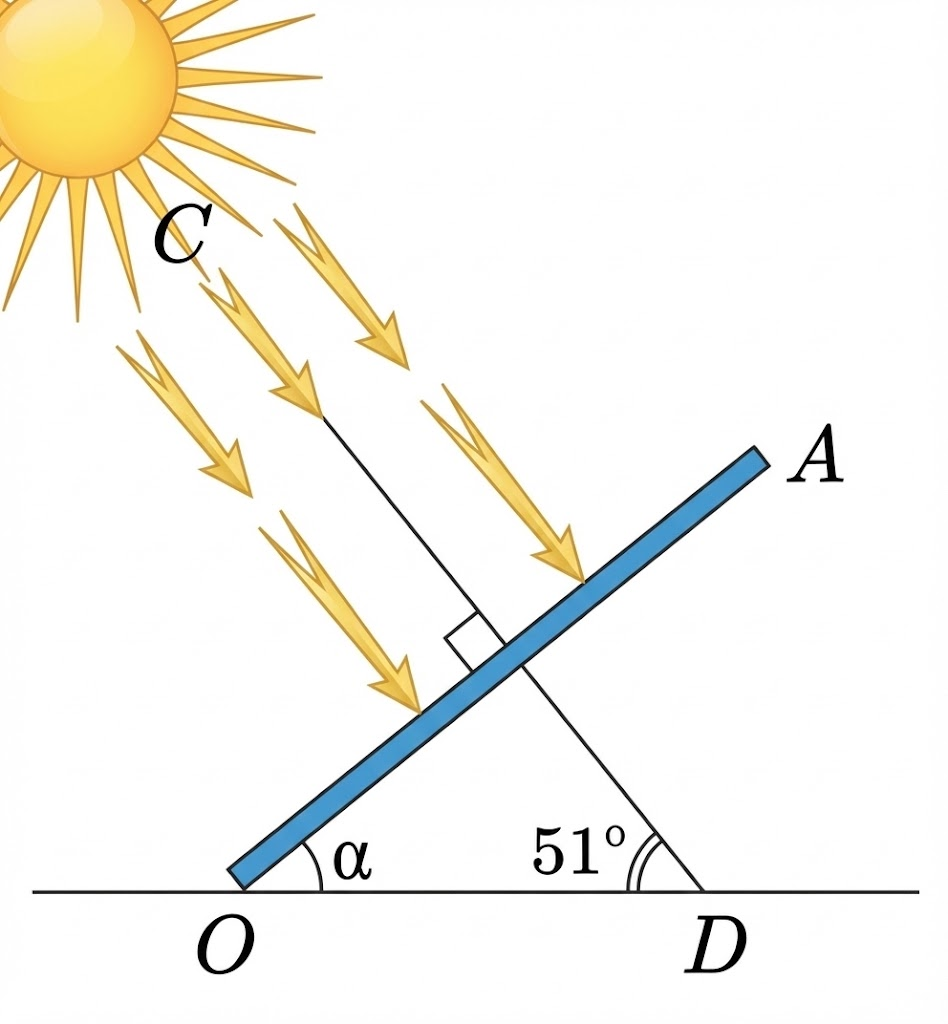
\includegraphics[scale=0.15]{solar_panel.png}
\end{flushright}
\end{minipage}

\nmtnobreak
\nopagebreak\nbvspace{0.7cm}

\nmtnobreak
\par\penalty-20\vspace{0.25cm}
\end{samepage}
\endgroup

\begingroup
% --- макроси, перенесені зі старого файлу теми ---
\providecommand{\matchingLayout}{}\renewcommand{\matchingLayout}[3]{
    \noindent
    \begin{minipage}[t]{0.36\textwidth}\vspace{0pt}\raggedright
       
        #1
    \end{minipage}%
    \hfill
    \begin{minipage}[t]{0.43\textwidth}\vspace{0pt}\raggedright
        
        #2
    \end{minipage}%
    \hfill
    \begin{minipage}[t]{0.19\textwidth}\vspace{0pt}\raggedright
        \vspace{0pt} % Хаки для вирівнювання minipage по верху
        \begin{flushright}
        #3
        \end{flushright}
    \end{minipage}
}

% --- сумісність зі старою базою (діє, якщо тема не має власного визначення) ---
\providecommand{\trigStyle}[1]{#1}
\providecommand{\answerTableSmall}[5]{%
\begingroup\setlength{\tabcolsep}{2pt}\small\nmtSetCell
\begin{tabular}{|*{5}{>{\centering\arraybackslash}m{\nmtcellw}|}}
\hline
\rule[-0.2cm]{0pt}{0.6cm}\textbf{А} & \textbf{Б} & \textbf{В} & \textbf{Г} & \textbf{Д} \\
\hline
\rule[-0.4cm]{0pt}{0.9cm}#1 & \rule[-0.4cm]{0pt}{0.9cm}#2 & \rule[-0.4cm]{0pt}{0.9cm}#3 & \rule[-0.4cm]{0pt}{0.9cm}#4 & \rule[-0.4cm]{0pt}{0.9cm}#5 \\
\hline
\end{tabular}\endgroup}
\providecommand{\matchingLayout}[3]{%
    \noindent
    \begin{minipage}[t]{0.36\textwidth}\vspace{0pt}\raggedright
        #1
    \end{minipage}%
    \hfill
    \begin{minipage}[t]{0.43\textwidth}\vspace{0pt}\raggedright
        #2
    \end{minipage}%
    \hfill
    \begin{minipage}[t]{0.19\textwidth}
        \vspace{0pt}
        \begin{flushright}
        #3
        \end{flushright}
    \end{minipage}}
\providecommand{\matchingLayoutBottom}[2]{%
    \noindent
    \begin{minipage}[t]{0.48\textwidth}\vspace{0pt}\raggedright
        #1
    \end{minipage}%
    \hfill
    \begin{minipage}[t]{0.48\textwidth}\vspace{0pt}\raggedright
        #2
    \end{minipage}
    \vspace{0.5cm}
    \noindent
    \matchingGrid}
\providecommand{\answerListVertical}[5]{%
    \par\nopagebreak\vspace{0.2cm}
    \begin{itemize}[itemsep=0.4cm, leftmargin=1.5cm, labelsep=0.5cm]
        \item[\textbf{А}] #1
        \item[\textbf{Б}] #2
        \item[\textbf{В}] #3
        \item[\textbf{Г}] #4
        \item[\textbf{Д}] #5
    \end{itemize}
    \vspace{0.2cm}}
\begin{samepage}
\noindent\zadnum Розв'яжіть нерівність $4(x - 2) \leqslant 2$.
\answerTable{$(-\infty; 1]$}{$[1; +\infty)$}{$(-\infty; 2{,}5]$}{$(-\infty; 1{,}5]$}{$[2{,}5; +\infty)$}
\par\penalty-20
\end{samepage}
\endgroup

\begingroup
% --- макроси з файлів сесій НМТ-2026 (для рисунків) ---
\renewcommand{\headrulewidth}{0.4pt}
\renewcommand{\footrulewidth}{0.4pt}

% --- сумісність зі старою базою (діє, якщо тема не має власного визначення) ---
\providecommand{\trigStyle}[1]{#1}
\providecommand{\answerTableSmall}[5]{%
\begingroup\setlength{\tabcolsep}{2pt}\small\nmtSetCell
\begin{tabular}{|*{5}{>{\centering\arraybackslash}m{\nmtcellw}|}}
\hline
\rule[-0.2cm]{0pt}{0.6cm}\textbf{А} & \textbf{Б} & \textbf{В} & \textbf{Г} & \textbf{Д} \\
\hline
\rule[-0.4cm]{0pt}{0.9cm}#1 & \rule[-0.4cm]{0pt}{0.9cm}#2 & \rule[-0.4cm]{0pt}{0.9cm}#3 & \rule[-0.4cm]{0pt}{0.9cm}#4 & \rule[-0.4cm]{0pt}{0.9cm}#5 \\
\hline
\end{tabular}\endgroup}
\providecommand{\matchingLayout}[3]{%
    \noindent
    \begin{minipage}[t]{0.36\textwidth}\vspace{0pt}\raggedright
        #1
    \end{minipage}%
    \hfill
    \begin{minipage}[t]{0.43\textwidth}\vspace{0pt}\raggedright
        #2
    \end{minipage}%
    \hfill
    \begin{minipage}[t]{0.19\textwidth}
        \vspace{0pt}
        \begin{flushright}
        #3
        \end{flushright}
    \end{minipage}}
\providecommand{\matchingLayoutBottom}[2]{%
    \noindent
    \begin{minipage}[t]{0.48\textwidth}\vspace{0pt}\raggedright
        #1
    \end{minipage}%
    \hfill
    \begin{minipage}[t]{0.48\textwidth}\vspace{0pt}\raggedright
        #2
    \end{minipage}
    \vspace{0.5cm}
    \noindent
    \matchingGrid}
\providecommand{\answerListVertical}[5]{%
    \par\nopagebreak\vspace{0.2cm}
    \begin{itemize}[itemsep=0.4cm, leftmargin=1.5cm, labelsep=0.5cm]
        \item[\textbf{А}] #1
        \item[\textbf{Б}] #2
        \item[\textbf{В}] #3
        \item[\textbf{Г}] #4
        \item[\textbf{Д}] #5
    \end{itemize}
    \vspace{0.2cm}}
\begin{samepage}
\noindent\zadnum \begin{minipage}[t]{0.55\textwidth}
На рисунку зображено чотирикутну піраміду $SABCD$. Скільки прямих, перпендикулярних до висоти $SO$, лежать в площині основи $ABCD$?

\nopagebreak\nbvspace{0.3cm}
\textbf{А} \quad жодної

\textbf{Б} \quad лише одна

\textbf{В} \quad лише дві

\textbf{Г} \quad лише три

\textbf{Д} \quad безліч
\end{minipage}
\hfill
\begin{minipage}[t]{0.40\textwidth}
\nopagebreak\nbvspace{-0.3cm}
\begin{center}
\begin{nmtfit}\begin{tikzpicture}[scale=0.9]
    %
    \coordinate (A) at (-2, -1);
    \coordinate (B) at (1.5, -1);
    \coordinate (C) at (2.5, 0.8);
    \coordinate (D) at (-1, 0.8);

    %
    \coordinate (O) at (0.25, -0.1); 
    \coordinate (S) at (0.25, 3.2); %

    %
    \draw[dashed] (A) -- (D) -- (C);
    \draw[dashed] (S) -- (D);

    %
    \draw[thick] (A) -- (B) -- (C);

    %
    \draw[thick] (S) -- (A);
    \draw[thick] (S) -- (B);
    \draw[thick] (S) -- (C);

    %
    \draw[dashed, gray] (A) -- (C);
    \draw[dashed, gray] (B) -- (D);
    \draw[dashed, thick] (S) -- (O); %

    %
    \node[below left] at (A) {$A$};
    \node[below right] at (B) {$B$};
    \node[right] at (C) {$C$};
    \node[left] at (D) {$D$};
    \node[above] at (S) {$S$};
    \node[below, font=\footnotesize, yshift=-2pt] at (O) {$O$};

    %
    \draw (O) -- ++(0, 0.25) -- ++(0.25, 0);

\end{tikzpicture}\end{nmtfit}
\end{center}
\end{minipage}

\nmtnobreak
\nopagebreak\nbvspace{0.5cm}
\par\penalty-20\vspace{0.25cm}
\end{samepage}
\endgroup

\begingroup
% --- сумісність зі старою базою (діє, якщо тема не має власного визначення) ---
\providecommand{\trigStyle}[1]{#1}
\providecommand{\answerTableSmall}[5]{%
\begingroup\setlength{\tabcolsep}{2pt}\small\nmtSetCell
\begin{tabular}{|*{5}{>{\centering\arraybackslash}m{\nmtcellw}|}}
\hline
\rule[-0.2cm]{0pt}{0.6cm}\textbf{А} & \textbf{Б} & \textbf{В} & \textbf{Г} & \textbf{Д} \\
\hline
\rule[-0.4cm]{0pt}{0.9cm}#1 & \rule[-0.4cm]{0pt}{0.9cm}#2 & \rule[-0.4cm]{0pt}{0.9cm}#3 & \rule[-0.4cm]{0pt}{0.9cm}#4 & \rule[-0.4cm]{0pt}{0.9cm}#5 \\
\hline
\end{tabular}\endgroup}
\providecommand{\matchingLayout}[3]{%
    \noindent
    \begin{minipage}[t]{0.36\textwidth}\vspace{0pt}\raggedright
        #1
    \end{minipage}%
    \hfill
    \begin{minipage}[t]{0.43\textwidth}\vspace{0pt}\raggedright
        #2
    \end{minipage}%
    \hfill
    \begin{minipage}[t]{0.19\textwidth}
        \vspace{0pt}
        \begin{flushright}
        #3
        \end{flushright}
    \end{minipage}}
\providecommand{\matchingLayoutBottom}[2]{%
    \noindent
    \begin{minipage}[t]{0.48\textwidth}\vspace{0pt}\raggedright
        #1
    \end{minipage}%
    \hfill
    \begin{minipage}[t]{0.48\textwidth}\vspace{0pt}\raggedright
        #2
    \end{minipage}
    \vspace{0.5cm}
    \noindent
    \matchingGrid}
\providecommand{\answerListVertical}[5]{%
    \par\nopagebreak\vspace{0.2cm}
    \begin{itemize}[itemsep=0.4cm, leftmargin=1.5cm, labelsep=0.5cm]
        \item[\textbf{А}] #1
        \item[\textbf{Б}] #2
        \item[\textbf{В}] #3
        \item[\textbf{Г}] #4
        \item[\textbf{Д}] #5
    \end{itemize}
    \vspace{0.2cm}}
\begin{samepage}
\zadtask{$(\sqrt{2} - a)(\sqrt{2} + a) =$}
\answerTable{$2 - a^2$}{$\sqrt[4]{2} - a^2$}{$2 - \sqrt{a}$}{$2 - a$}{$\sqrt{2} - a^2$}
\par\penalty-20
\end{samepage}
\endgroup

\begingroup
% --- макроси, перенесені зі старого файлу теми ---
\providecommand{\matchingLayout}{}\renewcommand{\matchingLayout}[3]{
    \noindent
    \begin{minipage}[t]{0.36\textwidth}\vspace{0pt}\raggedright
       
        #1
    \end{minipage}%
    \hfill
    \begin{minipage}[t]{0.43\textwidth}\vspace{0pt}\raggedright
        
        #2
    \end{minipage}%
    \hfill
    \begin{minipage}[t]{0.19\textwidth}\vspace{0pt}\raggedright
        \vspace{0pt} % Хаки для вирівнювання minipage по верху
        \begin{flushright}
        #3
        \end{flushright}
    \end{minipage}
}

% --- сумісність зі старою базою (діє, якщо тема не має власного визначення) ---
\providecommand{\trigStyle}[1]{#1}
\providecommand{\answerTableSmall}[5]{%
\begingroup\setlength{\tabcolsep}{2pt}\small\nmtSetCell
\begin{tabular}{|*{5}{>{\centering\arraybackslash}m{\nmtcellw}|}}
\hline
\rule[-0.2cm]{0pt}{0.6cm}\textbf{А} & \textbf{Б} & \textbf{В} & \textbf{Г} & \textbf{Д} \\
\hline
\rule[-0.4cm]{0pt}{0.9cm}#1 & \rule[-0.4cm]{0pt}{0.9cm}#2 & \rule[-0.4cm]{0pt}{0.9cm}#3 & \rule[-0.4cm]{0pt}{0.9cm}#4 & \rule[-0.4cm]{0pt}{0.9cm}#5 \\
\hline
\end{tabular}\endgroup}
\providecommand{\matchingLayout}[3]{%
    \noindent
    \begin{minipage}[t]{0.36\textwidth}\vspace{0pt}\raggedright
        #1
    \end{minipage}%
    \hfill
    \begin{minipage}[t]{0.43\textwidth}\vspace{0pt}\raggedright
        #2
    \end{minipage}%
    \hfill
    \begin{minipage}[t]{0.19\textwidth}
        \vspace{0pt}
        \begin{flushright}
        #3
        \end{flushright}
    \end{minipage}}
\providecommand{\matchingLayoutBottom}[2]{%
    \noindent
    \begin{minipage}[t]{0.48\textwidth}\vspace{0pt}\raggedright
        #1
    \end{minipage}%
    \hfill
    \begin{minipage}[t]{0.48\textwidth}\vspace{0pt}\raggedright
        #2
    \end{minipage}
    \vspace{0.5cm}
    \noindent
    \matchingGrid}
\providecommand{\answerListVertical}[5]{%
    \par\nopagebreak\vspace{0.2cm}
    \begin{itemize}[itemsep=0.4cm, leftmargin=1.5cm, labelsep=0.5cm]
        \item[\textbf{А}] #1
        \item[\textbf{Б}] #2
        \item[\textbf{В}] #3
        \item[\textbf{Г}] #4
        \item[\textbf{Д}] #5
    \end{itemize}
    \vspace{0.2cm}}
\begin{samepage}
\noindent\zadnum Розв'яжіть рівняння $3^x = 81 \cdot 9^x$.

\nmtnobreak
\answerTable{$4$}{$-4$}{$-2$}{$-3$}{$3$}
\par\penalty-20
\end{samepage}
\endgroup

\begingroup
% --- макроси, перенесені зі старого файлу теми ---
\providecommand{\matchingLayout}{}\renewcommand{\matchingLayout}[3]{
    \noindent
    \begin{minipage}[t]{0.36\textwidth}\vspace{0pt}\raggedright
       
        #1
    \end{minipage}%
    \hfill
    \begin{minipage}[t]{0.43\textwidth}\vspace{0pt}\raggedright
        
        #2
    \end{minipage}%
    \hfill
    \begin{minipage}[t]{0.19\textwidth}\vspace{0pt}\raggedright
        \vspace{0pt} % Хаки для вирівнювання minipage по верху
        \begin{flushright}
        #3
        \end{flushright}
    \end{minipage}
}

% --- макроси з файлів сесій НМТ-2026 (для рисунків) ---
\renewcommand{\headrulewidth}{0.4pt}
\renewcommand{\footrulewidth}{0.4pt}
\definecolor{gold}{RGB}{240, 190, 40}
\definecolor{silver}{RGB}{170, 170, 175}
\definecolor{bronze}{RGB}{190, 120, 70}
\definecolor{bar1}{RGB}{200, 120, 20}
\definecolor{bar2}{RGB}{255, 220, 0}
\definecolor{bar3}{RGB}{220, 30, 30}
\definecolor{bar4}{RGB}{128, 0, 128}
\definecolor{bar5}{RGB}{0, 160, 220}
\definecolor{bar6}{RGB}{120, 180, 50}
\definecolor{hexcol}{RGB}{200,110,60}
\providecommand{\hexthree}{}\renewcommand{\hexthree}[2]{%
    \draw[hexcol, line width=1.1pt]
        ($(#1,#2)+(0:30)$) -- ($(#1,#2)+(60:30)$) -- ($(#1,#2)+(120:30)$) --
        ($(#1,#2)+(180:30)$) -- ($(#1,#2)+(240:30)$) -- ($(#1,#2)+(300:30)$) -- cycle;
}

% --- сумісність зі старою базою (діє, якщо тема не має власного визначення) ---
\providecommand{\trigStyle}[1]{#1}
\providecommand{\answerTableSmall}[5]{%
\begingroup\setlength{\tabcolsep}{2pt}\small\nmtSetCell
\begin{tabular}{|*{5}{>{\centering\arraybackslash}m{\nmtcellw}|}}
\hline
\rule[-0.2cm]{0pt}{0.6cm}\textbf{А} & \textbf{Б} & \textbf{В} & \textbf{Г} & \textbf{Д} \\
\hline
\rule[-0.4cm]{0pt}{0.9cm}#1 & \rule[-0.4cm]{0pt}{0.9cm}#2 & \rule[-0.4cm]{0pt}{0.9cm}#3 & \rule[-0.4cm]{0pt}{0.9cm}#4 & \rule[-0.4cm]{0pt}{0.9cm}#5 \\
\hline
\end{tabular}\endgroup}
\providecommand{\matchingLayout}[3]{%
    \noindent
    \begin{minipage}[t]{0.36\textwidth}\vspace{0pt}\raggedright
        #1
    \end{minipage}%
    \hfill
    \begin{minipage}[t]{0.43\textwidth}\vspace{0pt}\raggedright
        #2
    \end{minipage}%
    \hfill
    \begin{minipage}[t]{0.19\textwidth}
        \vspace{0pt}
        \begin{flushright}
        #3
        \end{flushright}
    \end{minipage}}
\providecommand{\matchingLayoutBottom}[2]{%
    \noindent
    \begin{minipage}[t]{0.48\textwidth}\vspace{0pt}\raggedright
        #1
    \end{minipage}%
    \hfill
    \begin{minipage}[t]{0.48\textwidth}\vspace{0pt}\raggedright
        #2
    \end{minipage}
    \vspace{0.5cm}
    \noindent
    \matchingGrid}
\providecommand{\answerListVertical}[5]{%
    \par\nopagebreak\vspace{0.2cm}
    \begin{itemize}[itemsep=0.4cm, leftmargin=1.5cm, labelsep=0.5cm]
        \item[\textbf{А}] #1
        \item[\textbf{Б}] #2
        \item[\textbf{В}] #3
        \item[\textbf{Г}] #4
        \item[\textbf{Д}] #5
    \end{itemize}
    \vspace{0.2cm}}
\begin{samepage}
\zadtask{Задано функцію $f(x) = x^2$. Укажіть правильну нерівність.}
\answerTable{$f(4) < 0$}{$f(-4) < f(4)$}{$f(-1) > f(2)$}{$f(-1) < 0$}{$f(3) < f(4)$}

\par\penalty-20
\end{samepage}
\endgroup

\begingroup
% --- макроси, перенесені зі старого файлу теми ---
\providecommand{\matchingLayout}{}\renewcommand{\matchingLayout}[3]{
    \noindent
    \begin{minipage}[t]{0.36\textwidth}\vspace{0pt}\raggedright
       
        #1
    \end{minipage}%
    \hfill
    \begin{minipage}[t]{0.43\textwidth}\vspace{0pt}\raggedright
        
        #2
    \end{minipage}%
    \hfill
    \begin{minipage}[t]{0.19\textwidth}\vspace{0pt}\raggedright
        \vspace{0pt} % Хаки для вирівнювання minipage по верху
        \begin{flushright}
        #3
        \end{flushright}
    \end{minipage}
}

% --- макроси з файлів сесій НМТ-2026 (для рисунків) ---
\renewcommand{\headrulewidth}{0.4pt}
\renewcommand{\footrulewidth}{0.4pt}
\definecolor{bar1}{RGB}{200, 120, 20}
\definecolor{bar2}{RGB}{255, 220, 0}
\definecolor{bar3}{RGB}{220, 30, 30}
\definecolor{bar4}{RGB}{128, 0, 128}
\definecolor{bar5}{RGB}{0, 160, 220}
\definecolor{bar6}{RGB}{120, 180, 50}

% --- сумісність зі старою базою (діє, якщо тема не має власного визначення) ---
\providecommand{\trigStyle}[1]{#1}
\providecommand{\answerTableSmall}[5]{%
\begingroup\setlength{\tabcolsep}{2pt}\small\nmtSetCell
\begin{tabular}{|*{5}{>{\centering\arraybackslash}m{\nmtcellw}|}}
\hline
\rule[-0.2cm]{0pt}{0.6cm}\textbf{А} & \textbf{Б} & \textbf{В} & \textbf{Г} & \textbf{Д} \\
\hline
\rule[-0.4cm]{0pt}{0.9cm}#1 & \rule[-0.4cm]{0pt}{0.9cm}#2 & \rule[-0.4cm]{0pt}{0.9cm}#3 & \rule[-0.4cm]{0pt}{0.9cm}#4 & \rule[-0.4cm]{0pt}{0.9cm}#5 \\
\hline
\end{tabular}\endgroup}
\providecommand{\matchingLayout}[3]{%
    \noindent
    \begin{minipage}[t]{0.36\textwidth}\vspace{0pt}\raggedright
        #1
    \end{minipage}%
    \hfill
    \begin{minipage}[t]{0.43\textwidth}\vspace{0pt}\raggedright
        #2
    \end{minipage}%
    \hfill
    \begin{minipage}[t]{0.19\textwidth}
        \vspace{0pt}
        \begin{flushright}
        #3
        \end{flushright}
    \end{minipage}}
\providecommand{\matchingLayoutBottom}[2]{%
    \noindent
    \begin{minipage}[t]{0.48\textwidth}\vspace{0pt}\raggedright
        #1
    \end{minipage}%
    \hfill
    \begin{minipage}[t]{0.48\textwidth}\vspace{0pt}\raggedright
        #2
    \end{minipage}
    \vspace{0.5cm}
    \noindent
    \matchingGrid}
\providecommand{\answerListVertical}[5]{%
    \par\nopagebreak\vspace{0.2cm}
    \begin{itemize}[itemsep=0.4cm, leftmargin=1.5cm, labelsep=0.5cm]
        \item[\textbf{А}] #1
        \item[\textbf{Б}] #2
        \item[\textbf{В}] #3
        \item[\textbf{Г}] #4
        \item[\textbf{Д}] #5
    \end{itemize}
    \vspace{0.2cm}}
\begin{samepage}
\zadtask{Які з наведених тверджень щодо кола є правильними?\par
\nopagebreak\nbvspace{0.1cm}
\begin{enumerate}[label=\textbf{\Roman*.}, align=left, leftmargin=2.6em, labelsep=0.5em, itemsep=2pt, topsep=2pt]
\item Дуга кола~--- це відрізок, який сполучає $2$ точки на колі.
\item Центральний кут~--- це кут, вершина якого лежить на колі.
\item Вписаний кут, що спирається на діаметр,~--- прямий.
\end{enumerate}
\nopagebreak\nbvspace{0.1cm}}
\answerTable{лише I}{лише II}{лише III}{лише I та III}{лише II та III}
\par\penalty-20
\end{samepage}
\endgroup

\begingroup
% --- макроси з файлів сесій НМТ-2026 (для рисунків) ---
\renewcommand{\headrulewidth}{0.4pt}
\renewcommand{\footrulewidth}{0.4pt}

% --- сумісність зі старою базою (діє, якщо тема не має власного визначення) ---
\providecommand{\trigStyle}[1]{#1}
\providecommand{\answerTableSmall}[5]{%
\begingroup\setlength{\tabcolsep}{2pt}\small\nmtSetCell
\begin{tabular}{|*{5}{>{\centering\arraybackslash}m{\nmtcellw}|}}
\hline
\rule[-0.2cm]{0pt}{0.6cm}\textbf{А} & \textbf{Б} & \textbf{В} & \textbf{Г} & \textbf{Д} \\
\hline
\rule[-0.4cm]{0pt}{0.9cm}#1 & \rule[-0.4cm]{0pt}{0.9cm}#2 & \rule[-0.4cm]{0pt}{0.9cm}#3 & \rule[-0.4cm]{0pt}{0.9cm}#4 & \rule[-0.4cm]{0pt}{0.9cm}#5 \\
\hline
\end{tabular}\endgroup}
\providecommand{\matchingLayout}[3]{%
    \noindent
    \begin{minipage}[t]{0.36\textwidth}\vspace{0pt}\raggedright
        #1
    \end{minipage}%
    \hfill
    \begin{minipage}[t]{0.43\textwidth}\vspace{0pt}\raggedright
        #2
    \end{minipage}%
    \hfill
    \begin{minipage}[t]{0.19\textwidth}
        \vspace{0pt}
        \begin{flushright}
        #3
        \end{flushright}
    \end{minipage}}
\providecommand{\matchingLayoutBottom}[2]{%
    \noindent
    \begin{minipage}[t]{0.48\textwidth}\vspace{0pt}\raggedright
        #1
    \end{minipage}%
    \hfill
    \begin{minipage}[t]{0.48\textwidth}\vspace{0pt}\raggedright
        #2
    \end{minipage}
    \vspace{0.5cm}
    \noindent
    \matchingGrid}
\providecommand{\answerListVertical}[5]{%
    \par\nopagebreak\vspace{0.2cm}
    \begin{itemize}[itemsep=0.4cm, leftmargin=1.5cm, labelsep=0.5cm]
        \item[\textbf{А}] #1
        \item[\textbf{Б}] #2
        \item[\textbf{В}] #3
        \item[\textbf{Г}] #4
        \item[\textbf{Д}] #5
    \end{itemize}
    \vspace{0.2cm}}
\begin{samepage}
\noindent\zadnum \begin{minipage}[t]{0.55\textwidth}
На рисунку зображено графік функції $y=f(x)$, визначеної на проміжку $[-5; 5]$. Укажіть абсцису $x_0$ точки, у якій дотична до графіка функції, паралельна до осі $x$.
\end{minipage}
\hfill
\begin{minipage}[t]{0.40\textwidth}
\nopagebreak\nbvspace{-0.3cm}
\begin{center}
\begin{nmtfit}\begin{tikzpicture}
    \begin{axis}[
        x=0.5cm, y=0.5cm,
        axis lines=middle,
        xmin=-6, xmax=6,
        ymin=-2, ymax=6,
        xlabel={$x$}, ylabel={$y$},
        grid=both,
        grid style={line width=.2pt, draw=gray!40},
        xtick={-6,-5,...,6},
        ytick={-2,-1,...,6},
        ticklabel style={font=\footnotesize},
        xticklabels={,-5,,,,,0,1,,,,5,},
        yticklabels={,,0,1,,,,,,}, 
        clip=false
    ]
        %
        \addplot[thick, smooth, tension=0.6] coordinates {
            (-5, -1.5) 
            (-3.5, 2.5)
            (-2, 4.2)   %
            (-0.5, 2.5)
            (1, 1)      %
            (3, 3)
            (5, 5.5)
        };

        \addplot[only marks, mark=*] coordinates {(-5,-1.5) (5, 5.5)};
        \node[right, fill=white, inner sep=1.5pt] at (axis cs:1.5, 4.5) {$y=f(x)$};
    \end{axis}
\end{tikzpicture}\end{nmtfit}
\end{center}
\end{minipage}

\nmtnobreak
\nopagebreak\nbvspace{0.3cm}
\answerTable{$-3$}{$7$}{$1$}{$3$}{$-1$}
\par\penalty-20
\end{samepage}
\endgroup

\begingroup
% --- макроси з файлів сесій НМТ-2026 (для рисунків) ---
\renewcommand{\headrulewidth}{0.4pt}
\renewcommand{\footrulewidth}{0.4pt}
\definecolor{gold}{RGB}{240, 190, 40}
\definecolor{silver}{RGB}{170, 170, 175}
\definecolor{bronze}{RGB}{190, 120, 70}

% --- сумісність зі старою базою (діє, якщо тема не має власного визначення) ---
\providecommand{\trigStyle}[1]{#1}
\providecommand{\answerTableSmall}[5]{%
\begingroup\setlength{\tabcolsep}{2pt}\small\nmtSetCell
\begin{tabular}{|*{5}{>{\centering\arraybackslash}m{\nmtcellw}|}}
\hline
\rule[-0.2cm]{0pt}{0.6cm}\textbf{А} & \textbf{Б} & \textbf{В} & \textbf{Г} & \textbf{Д} \\
\hline
\rule[-0.4cm]{0pt}{0.9cm}#1 & \rule[-0.4cm]{0pt}{0.9cm}#2 & \rule[-0.4cm]{0pt}{0.9cm}#3 & \rule[-0.4cm]{0pt}{0.9cm}#4 & \rule[-0.4cm]{0pt}{0.9cm}#5 \\
\hline
\end{tabular}\endgroup}
\providecommand{\matchingLayout}[3]{%
    \noindent
    \begin{minipage}[t]{0.36\textwidth}\vspace{0pt}\raggedright
        #1
    \end{minipage}%
    \hfill
    \begin{minipage}[t]{0.43\textwidth}\vspace{0pt}\raggedright
        #2
    \end{minipage}%
    \hfill
    \begin{minipage}[t]{0.19\textwidth}
        \vspace{0pt}
        \begin{flushright}
        #3
        \end{flushright}
    \end{minipage}}
\providecommand{\matchingLayoutBottom}[2]{%
    \noindent
    \begin{minipage}[t]{0.48\textwidth}\vspace{0pt}\raggedright
        #1
    \end{minipage}%
    \hfill
    \begin{minipage}[t]{0.48\textwidth}\vspace{0pt}\raggedright
        #2
    \end{minipage}
    \vspace{0.5cm}
    \noindent
    \matchingGrid}
\providecommand{\answerListVertical}[5]{%
    \par\nopagebreak\vspace{0.2cm}
    \begin{itemize}[itemsep=0.4cm, leftmargin=1.5cm, labelsep=0.5cm]
        \item[\textbf{А}] #1
        \item[\textbf{Б}] #2
        \item[\textbf{В}] #3
        \item[\textbf{Г}] #4
        \item[\textbf{Д}] #5
    \end{itemize}
    \vspace{0.2cm}}
\begin{samepage}
\noindent\zadnum Комп’ютерна програма видаляє у шестицифровому числі одну цифру навмання. Яка \textbf{ймовірність} того, що в числі 125790 буде видалено непарну цифру?

\nmtnobreak
\nopagebreak\nbvspace{0.3cm}
\answerTableTall{$\dfrac{2}{3}$}{$\dfrac{1}{2}$}{$\dfrac{1}{3}$}{$\dfrac{5}{6}$}{$\dfrac{1}{6}$}
\par\penalty-20
\end{samepage}
\endgroup

\begingroup
% --- макроси, перенесені зі старого файлу теми ---
\providecommand{\matchingLayout}{}\renewcommand{\matchingLayout}[3]{
    \noindent
    \begin{minipage}[t]{0.36\textwidth}\vspace{0pt}\raggedright
       
        #1
    \end{minipage}%
    \hfill
    \begin{minipage}[t]{0.43\textwidth}\vspace{0pt}\raggedright
        
        #2
    \end{minipage}%
    \hfill
    \begin{minipage}[t]{0.19\textwidth}\vspace{0pt}\raggedright
        \vspace{0pt} % Хаки для вирівнювання minipage по верху
        \begin{flushright}
        #3
        \end{flushright}
    \end{minipage}
}

% --- макроси з файлів сесій НМТ-2026 (для рисунків) ---
\renewcommand{\headrulewidth}{0.4pt}
\renewcommand{\footrulewidth}{0.4pt}
\definecolor{hexcol}{RGB}{200,110,60}
\providecommand{\hexthree}{}\renewcommand{\hexthree}[2]{%
    \draw[hexcol, line width=1.1pt]
        ($(#1,#2)+(0:30)$) -- ($(#1,#2)+(60:30)$) -- ($(#1,#2)+(120:30)$) --
        ($(#1,#2)+(180:30)$) -- ($(#1,#2)+(240:30)$) -- ($(#1,#2)+(300:30)$) -- cycle;
}

% --- сумісність зі старою базою (діє, якщо тема не має власного визначення) ---
\providecommand{\trigStyle}[1]{#1}
\providecommand{\answerTableSmall}[5]{%
\begingroup\setlength{\tabcolsep}{2pt}\small\nmtSetCell
\begin{tabular}{|*{5}{>{\centering\arraybackslash}m{\nmtcellw}|}}
\hline
\rule[-0.2cm]{0pt}{0.6cm}\textbf{А} & \textbf{Б} & \textbf{В} & \textbf{Г} & \textbf{Д} \\
\hline
\rule[-0.4cm]{0pt}{0.9cm}#1 & \rule[-0.4cm]{0pt}{0.9cm}#2 & \rule[-0.4cm]{0pt}{0.9cm}#3 & \rule[-0.4cm]{0pt}{0.9cm}#4 & \rule[-0.4cm]{0pt}{0.9cm}#5 \\
\hline
\end{tabular}\endgroup}
\providecommand{\matchingLayout}[3]{%
    \noindent
    \begin{minipage}[t]{0.36\textwidth}\vspace{0pt}\raggedright
        #1
    \end{minipage}%
    \hfill
    \begin{minipage}[t]{0.43\textwidth}\vspace{0pt}\raggedright
        #2
    \end{minipage}%
    \hfill
    \begin{minipage}[t]{0.19\textwidth}
        \vspace{0pt}
        \begin{flushright}
        #3
        \end{flushright}
    \end{minipage}}
\providecommand{\matchingLayoutBottom}[2]{%
    \noindent
    \begin{minipage}[t]{0.48\textwidth}\vspace{0pt}\raggedright
        #1
    \end{minipage}%
    \hfill
    \begin{minipage}[t]{0.48\textwidth}\vspace{0pt}\raggedright
        #2
    \end{minipage}
    \vspace{0.5cm}
    \noindent
    \matchingGrid}
\providecommand{\answerListVertical}[5]{%
    \par\nopagebreak\vspace{0.2cm}
    \begin{itemize}[itemsep=0.4cm, leftmargin=1.5cm, labelsep=0.5cm]
        \item[\textbf{А}] #1
        \item[\textbf{Б}] #2
        \item[\textbf{В}] #3
        \item[\textbf{Г}] #4
        \item[\textbf{Д}] #5
    \end{itemize}
    \vspace{0.2cm}}
\begin{samepage}
\noindent\zadnum \begin{minipage}[t]{0.55\textwidth}
У прямокутній системі координат у просторі зображено прямокутний паралелепіпед, одна з вершин якого збігається з початком координат --- точкою $O$, а три ребра лежать на координатних осях (див. рисунок). Точка $K(12; 15; 16)$ є вершиною паралелепіпеда. Визначте довжину (модуль) вектора $\vec{OK}$.
\end{minipage}
\hfill
\begin{minipage}[t]{0.4\textwidth}
    \nopagebreak\nbvspace{-0.3cm}
    \begin{flushright}
    %
    \begin{nmtfit}\begin{tikzpicture}[x={(-0.5cm,-0.4cm)}, y={(0.8cm,0cm)}, z={(0cm,0.8cm)}, scale=0.15]

        %
        \coordinate (O) at (0,0,0);
        \coordinate (K) at (12,15,16);

        %
        \def\xk{12}
        \def\yk{15}
        \def\zk{16}

        %
        \coordinate (A) at (\xk,0,0);
        \coordinate (B) at (0,\yk,0);
        \coordinate (C) at (0,0,\zk);
        \coordinate (XY) at (\xk,\yk,0);
        \coordinate (XZ) at (\xk,0,\zk);
        \coordinate (YZ) at (0,\yk,\zk);

        %
        \draw[->, >=stealth] (0,0,0) -- (\xk+5,0,0) node[below left] {$x$};
        \draw[->, >=stealth] (0,0,0) -- (0,\yk+5,0) node[right] {$y$};
        \draw[->, >=stealth] (0,0,0) -- (0,0,\zk+5) node[left] {$z$};

        %
        \draw[dashed] (A) -- (XY) -- (B);
        \draw[dashed] (XY) -- (K);

        %
        \draw[thick] (O) -- (A) -- (XZ) -- (C) -- cycle; %
        \draw[thick] (O) -- (B) -- (YZ) -- (C) -- cycle; %
        %

        %
        %
        %

        %
        \draw[thick] (O) -- (A);
        \draw[thick] (O) -- (B);
        \draw[thick] (O) -- (C);

        \draw[thick] (A) -- (XZ);
        \draw[thick] (C) -- (XZ);
        \draw[thick] (C) -- (YZ);
        \draw[thick] (B) -- (YZ);
        \draw[thick] (XZ) -- (K);
        \draw[thick] (YZ) -- (K);

        %
        \draw[thick] (A) -- (XY) -- (B);
        \draw[thick] (XY) -- (K);

        %

        %
        \node[below right] at (O) {$O$};
        \node[above] at (K) {$K$};
        \fill (O) circle (8pt);
        \fill (K) circle (8pt);

    \end{tikzpicture}\end{nmtfit}
    \end{flushright}
\end{minipage}

\nmtnobreak
\nopagebreak\nbvspace{0.3cm}
\answerTable{$25$}{$43$}{$\sqrt{337}$}{$\sqrt{86}$}{$11$}
\par\penalty-20
\end{samepage}
\endgroup

\begingroup
% --- макроси, перенесені зі старого файлу теми ---
\providecommand{\matchingLayout}{}\renewcommand{\matchingLayout}[3]{
    \noindent
    \begin{minipage}[t]{0.36\textwidth}\vspace{0pt}\raggedright
       
        #1
    \end{minipage}%
    \hfill
    \begin{minipage}[t]{0.43\textwidth}\vspace{0pt}\raggedright
        
        #2
    \end{minipage}%
    \hfill
    \begin{minipage}[t]{0.19\textwidth}\vspace{0pt}\raggedright
        \vspace{0pt} % Хаки для вирівнювання minipage по верху
        \begin{flushright}
        #3
        \end{flushright}
    \end{minipage}
}
\providecommand{\trigStyle}{}\renewcommand{\trigStyle}[1]{\textbf{#1}}

% --- сумісність зі старою базою (діє, якщо тема не має власного визначення) ---
\providecommand{\trigStyle}[1]{#1}
\providecommand{\answerTableSmall}[5]{%
\begingroup\setlength{\tabcolsep}{2pt}\small\nmtSetCell
\begin{tabular}{|*{5}{>{\centering\arraybackslash}m{\nmtcellw}|}}
\hline
\rule[-0.2cm]{0pt}{0.6cm}\textbf{А} & \textbf{Б} & \textbf{В} & \textbf{Г} & \textbf{Д} \\
\hline
\rule[-0.4cm]{0pt}{0.9cm}#1 & \rule[-0.4cm]{0pt}{0.9cm}#2 & \rule[-0.4cm]{0pt}{0.9cm}#3 & \rule[-0.4cm]{0pt}{0.9cm}#4 & \rule[-0.4cm]{0pt}{0.9cm}#5 \\
\hline
\end{tabular}\endgroup}
\providecommand{\matchingLayout}[3]{%
    \noindent
    \begin{minipage}[t]{0.36\textwidth}\vspace{0pt}\raggedright
        #1
    \end{minipage}%
    \hfill
    \begin{minipage}[t]{0.43\textwidth}\vspace{0pt}\raggedright
        #2
    \end{minipage}%
    \hfill
    \begin{minipage}[t]{0.19\textwidth}
        \vspace{0pt}
        \begin{flushright}
        #3
        \end{flushright}
    \end{minipage}}
\providecommand{\matchingLayoutBottom}[2]{%
    \noindent
    \begin{minipage}[t]{0.48\textwidth}\vspace{0pt}\raggedright
        #1
    \end{minipage}%
    \hfill
    \begin{minipage}[t]{0.48\textwidth}\vspace{0pt}\raggedright
        #2
    \end{minipage}
    \vspace{0.5cm}
    \noindent
    \matchingGrid}
\providecommand{\answerListVertical}[5]{%
    \par\nopagebreak\vspace{0.2cm}
    \begin{itemize}[itemsep=0.4cm, leftmargin=1.5cm, labelsep=0.5cm]
        \item[\textbf{А}] #1
        \item[\textbf{Б}] #2
        \item[\textbf{В}] #3
        \item[\textbf{Г}] #4
        \item[\textbf{Д}] #5
    \end{itemize}
    \vspace{0.2cm}}
\begin{samepage}
\noindent\zadnum \trigStyle{$\dfrac{\cos(540^\circ - \alpha)}{\sin \alpha} = $}

\nmtnobreak
\nopagebreak\nbvspace{0.3cm}
\answerTableTall{$\dfrac{1}{\operatorname{tg} \alpha}$}{$-1$}{$1$}{$-\operatorname{tg} \alpha$}{$-\dfrac{1}{\operatorname{tg} \alpha}$}
\par\penalty-20
\end{samepage}
\endgroup

\begingroup
% --- макроси, перенесені зі старого файлу теми ---
\providecommand{\matchingLayout}{}\renewcommand{\matchingLayout}[3]{
    \noindent
    \begin{minipage}[t]{0.36\textwidth}\vspace{0pt}\raggedright
        #1
    \end{minipage}%
    \hfill
    \begin{minipage}[t]{0.43\textwidth}\vspace{0pt}\raggedright
        #2
    \end{minipage}%
    \hfill
    \begin{minipage}[t]{0.19\textwidth}\vspace{0pt}\raggedright
        \vspace{0pt} 
        \begin{flushright}
        #3
        \end{flushright}
    \end{minipage}
}

% --- макроси з файлів сесій НМТ-2026 (для рисунків) ---
\renewcommand{\headrulewidth}{0.4pt}
\renewcommand{\footrulewidth}{0.4pt}
\definecolor{gold}{RGB}{240, 190, 40}
\definecolor{silver}{RGB}{170, 170, 175}
\definecolor{bronze}{RGB}{190, 120, 70}
\definecolor{bar1}{RGB}{200, 120, 20}
\definecolor{bar2}{RGB}{255, 220, 0}
\definecolor{bar3}{RGB}{220, 30, 30}
\definecolor{bar4}{RGB}{128, 0, 128}
\definecolor{bar5}{RGB}{0, 160, 220}
\definecolor{bar6}{RGB}{120, 180, 50}

% --- сумісність зі старою базою (діє, якщо тема не має власного визначення) ---
\providecommand{\trigStyle}[1]{#1}
\providecommand{\answerTableSmall}[5]{%
\begingroup\setlength{\tabcolsep}{2pt}\small\nmtSetCell
\begin{tabular}{|*{5}{>{\centering\arraybackslash}m{\nmtcellw}|}}
\hline
\rule[-0.2cm]{0pt}{0.6cm}\textbf{А} & \textbf{Б} & \textbf{В} & \textbf{Г} & \textbf{Д} \\
\hline
\rule[-0.4cm]{0pt}{0.9cm}#1 & \rule[-0.4cm]{0pt}{0.9cm}#2 & \rule[-0.4cm]{0pt}{0.9cm}#3 & \rule[-0.4cm]{0pt}{0.9cm}#4 & \rule[-0.4cm]{0pt}{0.9cm}#5 \\
\hline
\end{tabular}\endgroup}
\providecommand{\matchingLayout}[3]{%
    \noindent
    \begin{minipage}[t]{0.36\textwidth}\vspace{0pt}\raggedright
        #1
    \end{minipage}%
    \hfill
    \begin{minipage}[t]{0.43\textwidth}\vspace{0pt}\raggedright
        #2
    \end{minipage}%
    \hfill
    \begin{minipage}[t]{0.19\textwidth}
        \vspace{0pt}
        \begin{flushright}
        #3
        \end{flushright}
    \end{minipage}}
\providecommand{\matchingLayoutBottom}[2]{%
    \noindent
    \begin{minipage}[t]{0.48\textwidth}\vspace{0pt}\raggedright
        #1
    \end{minipage}%
    \hfill
    \begin{minipage}[t]{0.48\textwidth}\vspace{0pt}\raggedright
        #2
    \end{minipage}
    \vspace{0.5cm}
    \noindent
    \matchingGrid}
\providecommand{\answerListVertical}[5]{%
    \par\nopagebreak\vspace{0.2cm}
    \begin{itemize}[itemsep=0.4cm, leftmargin=1.5cm, labelsep=0.5cm]
        \item[\textbf{А}] #1
        \item[\textbf{Б}] #2
        \item[\textbf{В}] #3
        \item[\textbf{Г}] #4
        \item[\textbf{Д}] #5
    \end{itemize}
    \vspace{0.2cm}}
\begin{samepage}
\noindent\zadnum \begin{minipage}[t]{0.55\textwidth}
Діагоналі прямокутника $ABCD$ перетинаються в точці $O$, $AB = 6$, $\angle AOD = 110^\circ$ (див. рисунок). Знайдіть периметр цього прямокутника.
\end{minipage}
\hfill
\begin{minipage}[t]{0.4\textwidth}
    \nopagebreak\nbvspace{-0.3cm}
    \begin{flushright}
    \begin{nmtfit}\begin{tikzpicture}[scale=0.6]
        \coordinate (A) at (0,0);
        \coordinate (B) at (0,3.5);
        \coordinate (C) at (6,3.5);
        \coordinate (D) at (6,0);
        \coordinate (O) at (3, 1.75);

        \draw[thick] (A) -- (B) -- (C) -- (D) -- cycle;
        \draw[thick] (A) -- (C);
        \draw[thick] (B) -- (D);

        %
        \pic [draw, pic text={\small $110^\circ$}, angle radius=0.5cm, angle eccentricity=1.5] {angle = A--O--D};

        \node[below left] at (A) {$A$};
        \node[above left] at (B) {$B$};
        \node[above right] at (C) {$C$};
        \node[below right] at (D) {$D$};
        \node[above] at (O) {$O$};
    \end{tikzpicture}\end{nmtfit}
    \end{flushright}
\end{minipage}

\nmtnobreak
\nopagebreak\nbvspace{0.3cm}
\noindent
\begin{tabular}{ll}
\textbf{А} & $6 + 6\tg 55^\circ$ \\[0.3cm]
\textbf{Б} & $12 + 12\sin 55^\circ$ \\[0.3cm]
\textbf{В} & $12 + \dfrac{12}{\tg 55^\circ}$ \\[0.5cm]
\textbf{Г} & $12 + 12\tg 55^\circ$ \\[0.3cm]
\textbf{Д} & $12 + 12\cos 55^\circ$
\end{tabular}
\par\penalty-20\vspace{0.25cm}
\end{samepage}
\endgroup

\begingroup
% --- макроси, перенесені зі старого файлу теми ---
\providecommand{\matchingLayout}{}\renewcommand{\matchingLayout}[3]{
    \noindent
    \begin{minipage}[t]{0.36\textwidth}\vspace{0pt}\raggedright
       
        #1
    \end{minipage}%
    \hfill
    \begin{minipage}[t]{0.43\textwidth}\vspace{0pt}\raggedright
        
        #2
    \end{minipage}%
    \hfill
    \begin{minipage}[t]{0.19\textwidth}\vspace{0pt}\raggedright
        \vspace{0pt} % Хаки для вирівнювання minipage по верху
        \begin{flushright}
        #3
        \end{flushright}
    \end{minipage}
}

% --- сумісність зі старою базою (діє, якщо тема не має власного визначення) ---
\providecommand{\trigStyle}[1]{#1}
\providecommand{\answerTableSmall}[5]{%
\begingroup\setlength{\tabcolsep}{2pt}\small\nmtSetCell
\begin{tabular}{|*{5}{>{\centering\arraybackslash}m{\nmtcellw}|}}
\hline
\rule[-0.2cm]{0pt}{0.6cm}\textbf{А} & \textbf{Б} & \textbf{В} & \textbf{Г} & \textbf{Д} \\
\hline
\rule[-0.4cm]{0pt}{0.9cm}#1 & \rule[-0.4cm]{0pt}{0.9cm}#2 & \rule[-0.4cm]{0pt}{0.9cm}#3 & \rule[-0.4cm]{0pt}{0.9cm}#4 & \rule[-0.4cm]{0pt}{0.9cm}#5 \\
\hline
\end{tabular}\endgroup}
\providecommand{\matchingLayout}[3]{%
    \noindent
    \begin{minipage}[t]{0.36\textwidth}\vspace{0pt}\raggedright
        #1
    \end{minipage}%
    \hfill
    \begin{minipage}[t]{0.43\textwidth}\vspace{0pt}\raggedright
        #2
    \end{minipage}%
    \hfill
    \begin{minipage}[t]{0.19\textwidth}
        \vspace{0pt}
        \begin{flushright}
        #3
        \end{flushright}
    \end{minipage}}
\providecommand{\matchingLayoutBottom}[2]{%
    \noindent
    \begin{minipage}[t]{0.48\textwidth}\vspace{0pt}\raggedright
        #1
    \end{minipage}%
    \hfill
    \begin{minipage}[t]{0.48\textwidth}\vspace{0pt}\raggedright
        #2
    \end{minipage}
    \vspace{0.5cm}
    \noindent
    \matchingGrid}
\providecommand{\answerListVertical}[5]{%
    \par\nopagebreak\vspace{0.2cm}
    \begin{itemize}[itemsep=0.4cm, leftmargin=1.5cm, labelsep=0.5cm]
        \item[\textbf{А}] #1
        \item[\textbf{Б}] #2
        \item[\textbf{В}] #3
        \item[\textbf{Г}] #4
        \item[\textbf{Д}] #5
    \end{itemize}
    \vspace{0.2cm}}
\begin{samepage}
\zadtask{Розв'яжіть рівняння $|2x - 5| = 8$. Якщо рівняння має кілька коренів, визначте їхню \textit{суму}.}

\nmtnobreak
\answerTable{$-6{,}5$}{$5$}{$8$}{$-1{,}5$}{$6{,}5$}
\par\penalty-20
\end{samepage}
\endgroup

\instructionBox{У завданнях 16--18 до кожного з трьох рядків інформації, позначених цифрами, доберіть один правильний, на Вашу думку, варіант, позначений буквою.}

\begingroup
% --- сумісність зі старою базою (діє, якщо тема не має власного визначення) ---
\providecommand{\trigStyle}[1]{#1}
\providecommand{\answerTableSmall}[5]{%
\begingroup\setlength{\tabcolsep}{2pt}\small\nmtSetCell
\begin{tabular}{|*{5}{>{\centering\arraybackslash}m{\nmtcellw}|}}
\hline
\rule[-0.2cm]{0pt}{0.6cm}\textbf{А} & \textbf{Б} & \textbf{В} & \textbf{Г} & \textbf{Д} \\
\hline
\rule[-0.4cm]{0pt}{0.9cm}#1 & \rule[-0.4cm]{0pt}{0.9cm}#2 & \rule[-0.4cm]{0pt}{0.9cm}#3 & \rule[-0.4cm]{0pt}{0.9cm}#4 & \rule[-0.4cm]{0pt}{0.9cm}#5 \\
\hline
\end{tabular}\endgroup}
\providecommand{\matchingLayout}[3]{%
    \noindent
    \begin{minipage}[t]{0.36\textwidth}\vspace{0pt}\raggedright
        #1
    \end{minipage}%
    \hfill
    \begin{minipage}[t]{0.43\textwidth}\vspace{0pt}\raggedright
        #2
    \end{minipage}%
    \hfill
    \begin{minipage}[t]{0.19\textwidth}
        \vspace{0pt}
        \begin{flushright}
        #3
        \end{flushright}
    \end{minipage}}
\providecommand{\matchingLayoutBottom}[2]{%
    \noindent
    \begin{minipage}[t]{0.48\textwidth}\vspace{0pt}\raggedright
        #1
    \end{minipage}%
    \hfill
    \begin{minipage}[t]{0.48\textwidth}\vspace{0pt}\raggedright
        #2
    \end{minipage}
    \vspace{0.5cm}
    \noindent
    \matchingGrid}
\providecommand{\answerListVertical}[5]{%
    \par\nopagebreak\vspace{0.2cm}
    \begin{itemize}[itemsep=0.4cm, leftmargin=1.5cm, labelsep=0.5cm]
        \item[\textbf{А}] #1
        \item[\textbf{Б}] #2
        \item[\textbf{В}] #3
        \item[\textbf{Г}] #4
        \item[\textbf{Д}] #5
    \end{itemize}
    \vspace{0.2cm}}
\begin{samepage}
\zadtask{Узгодьте вираз \mbox{(1--3)} із твердженням про його значення \mbox{(А--Д)}, що є правильним для цього виразу.}

\nmtnobreak
\nopagebreak\nbvspace{0.3cm}
\matchingLayout{
\matchHead{Вираз}
\matchItem{1}{$\sqrt[3]{-27}$}
\matchItem{2}{$\dfrac{\sqrt{12}}{\sqrt{300}}$}

\nmtnobreak
\matchItem{3}{$(\sqrt{3} - 1)^2 + 2\sqrt{3}$}
}{
\matchHead{Твердження про значення виразу}
\matchItem{А}{є цілим від'ємним числом}
\matchItem{Б}{є ірраціональним додатним числом}
\matchItem{В}{є ірраціональним від'ємним числом}
\matchItem{Г}{є натуральним числом}
\matchItem{Д}{є раціональним нецілим числом}
}{
\matchingGrid
}
\par\penalty-20\vspace{0.25cm}
\end{samepage}
\endgroup

\begingroup
% --- макроси, перенесені зі старого файлу теми ---
\providecommand{\matchingLayout}{}\renewcommand{\matchingLayout}[3]{
    \noindent
    \begin{minipage}[t]{0.36\textwidth}\vspace{0pt}\raggedright
       
        #1
    \end{minipage}%
    \hfill
    \begin{minipage}[t]{0.43\textwidth}\vspace{0pt}\raggedright
        
        #2
    \end{minipage}%
    \hfill
    \begin{minipage}[t]{0.19\textwidth}\vspace{0pt}\raggedright
        \vspace{0pt} % Хаки для вирівнювання minipage по верху
        \begin{flushright}
        #3
        \end{flushright}
    \end{minipage}
}

% --- макроси з файлів сесій НМТ-2026 (для рисунків) ---
\renewcommand{\headrulewidth}{0.4pt}
\renewcommand{\footrulewidth}{0.4pt}

% --- сумісність зі старою базою (діє, якщо тема не має власного визначення) ---
\providecommand{\trigStyle}[1]{#1}
\providecommand{\answerTableSmall}[5]{%
\begingroup\setlength{\tabcolsep}{2pt}\small\nmtSetCell
\begin{tabular}{|*{5}{>{\centering\arraybackslash}m{\nmtcellw}|}}
\hline
\rule[-0.2cm]{0pt}{0.6cm}\textbf{А} & \textbf{Б} & \textbf{В} & \textbf{Г} & \textbf{Д} \\
\hline
\rule[-0.4cm]{0pt}{0.9cm}#1 & \rule[-0.4cm]{0pt}{0.9cm}#2 & \rule[-0.4cm]{0pt}{0.9cm}#3 & \rule[-0.4cm]{0pt}{0.9cm}#4 & \rule[-0.4cm]{0pt}{0.9cm}#5 \\
\hline
\end{tabular}\endgroup}
\providecommand{\matchingLayout}[3]{%
    \noindent
    \begin{minipage}[t]{0.36\textwidth}\vspace{0pt}\raggedright
        #1
    \end{minipage}%
    \hfill
    \begin{minipage}[t]{0.43\textwidth}\vspace{0pt}\raggedright
        #2
    \end{minipage}%
    \hfill
    \begin{minipage}[t]{0.19\textwidth}
        \vspace{0pt}
        \begin{flushright}
        #3
        \end{flushright}
    \end{minipage}}
\providecommand{\matchingLayoutBottom}[2]{%
    \noindent
    \begin{minipage}[t]{0.48\textwidth}\vspace{0pt}\raggedright
        #1
    \end{minipage}%
    \hfill
    \begin{minipage}[t]{0.48\textwidth}\vspace{0pt}\raggedright
        #2
    \end{minipage}
    \vspace{0.5cm}
    \noindent
    \matchingGrid}
\providecommand{\answerListVertical}[5]{%
    \par\nopagebreak\vspace{0.2cm}
    \begin{itemize}[itemsep=0.4cm, leftmargin=1.5cm, labelsep=0.5cm]
        \item[\textbf{А}] #1
        \item[\textbf{Б}] #2
        \item[\textbf{В}] #3
        \item[\textbf{Г}] #4
        \item[\textbf{Д}] #5
    \end{itemize}
    \vspace{0.2cm}}
\begin{samepage}
\noindent\zadnum Доберіть до функції \mbox{(1--3)} її властивість \mbox{(А--Д)}.

\nmtnobreak
\nopagebreak\nbvspace{0.3cm}

\nmtnobreak
\noindent
\matchingLayout{
\matchHead{Функція}
    \matchItem{1}{$y=2x-5$}
\matchItem{2}{$y=\log_3(x-5)$}
\matchItem{3}{$y=x^2-5$}
}{
\matchHead{Властивість функції}
    \matchItem{А}{графік функції має лише 2 точки перетину з осями координат}
\matchItem{Б}{областю значень функції є проміжок $[-5; +\infty)$}
\matchItem{В}{графік функції знаходиться лише в I та II координатних чвертях}
\matchItem{Г}{областю визначення функції є проміжок $(5; +\infty)$}
\matchItem{Д}{функція спадає на всій області визначення}
}{
\matchingGrid
}
\par\penalty-20\vspace{0.25cm}
\end{samepage}
\endgroup

\begingroup
% --- макроси з файлів сесій НМТ-2026 (для рисунків) ---
\renewcommand{\headrulewidth}{0.4pt}
\renewcommand{\footrulewidth}{0.4pt}
\definecolor{gold}{RGB}{240, 190, 40}
\definecolor{silver}{RGB}{170, 170, 175}
\definecolor{bronze}{RGB}{190, 120, 70}
\definecolor{hexcol}{RGB}{200,110,60}
\providecommand{\hexthree}{}\renewcommand{\hexthree}[2]{%
    \draw[hexcol, line width=1.1pt]
        ($(#1,#2)+(0:30)$) -- ($(#1,#2)+(60:30)$) -- ($(#1,#2)+(120:30)$) --
        ($(#1,#2)+(180:30)$) -- ($(#1,#2)+(240:30)$) -- ($(#1,#2)+(300:30)$) -- cycle;
}

% --- сумісність зі старою базою (діє, якщо тема не має власного визначення) ---
\providecommand{\trigStyle}[1]{#1}
\providecommand{\answerTableSmall}[5]{%
\begingroup\setlength{\tabcolsep}{2pt}\small\nmtSetCell
\begin{tabular}{|*{5}{>{\centering\arraybackslash}m{\nmtcellw}|}}
\hline
\rule[-0.2cm]{0pt}{0.6cm}\textbf{А} & \textbf{Б} & \textbf{В} & \textbf{Г} & \textbf{Д} \\
\hline
\rule[-0.4cm]{0pt}{0.9cm}#1 & \rule[-0.4cm]{0pt}{0.9cm}#2 & \rule[-0.4cm]{0pt}{0.9cm}#3 & \rule[-0.4cm]{0pt}{0.9cm}#4 & \rule[-0.4cm]{0pt}{0.9cm}#5 \\
\hline
\end{tabular}\endgroup}
\providecommand{\matchingLayout}[3]{%
    \noindent
    \begin{minipage}[t]{0.36\textwidth}\vspace{0pt}\raggedright
        #1
    \end{minipage}%
    \hfill
    \begin{minipage}[t]{0.43\textwidth}\vspace{0pt}\raggedright
        #2
    \end{minipage}%
    \hfill
    \begin{minipage}[t]{0.19\textwidth}
        \vspace{0pt}
        \begin{flushright}
        #3
        \end{flushright}
    \end{minipage}}
\providecommand{\matchingLayoutBottom}[2]{%
    \noindent
    \begin{minipage}[t]{0.48\textwidth}\vspace{0pt}\raggedright
        #1
    \end{minipage}%
    \hfill
    \begin{minipage}[t]{0.48\textwidth}\vspace{0pt}\raggedright
        #2
    \end{minipage}
    \vspace{0.5cm}
    \noindent
    \matchingGrid}
\providecommand{\answerListVertical}[5]{%
    \par\nopagebreak\vspace{0.2cm}
    \begin{itemize}[itemsep=0.4cm, leftmargin=1.5cm, labelsep=0.5cm]
        \item[\textbf{А}] #1
        \item[\textbf{Б}] #2
        \item[\textbf{В}] #3
        \item[\textbf{Г}] #4
        \item[\textbf{Д}] #5
    \end{itemize}
    \vspace{0.2cm}}
\begin{samepage}
\zadtask{На паралельних прямих $n$ і $m$ розміщено сторони прямокутника $ABCD$ й паралелограма $DKLM$, вершини $L$ і $Q$ трикутника $LQP$ (див. рисунок). $BC = KL = 6$ \textit{см}, $AB : BC = 4 : 3$, $LP = PQ$, $\angle LPQ = 60°$, діагональ $KM$ паралелограма й сторона $LQ$ трикутника $LPQ$ перпендикулярні до прямої $n$. Установіть відповідність між фігурою \mbox{(1--3)} та її периметром \mbox{(А--Д)}.}

\nmtnobreak
\nopagebreak\nbvspace{0.3cm}
\begin{center}
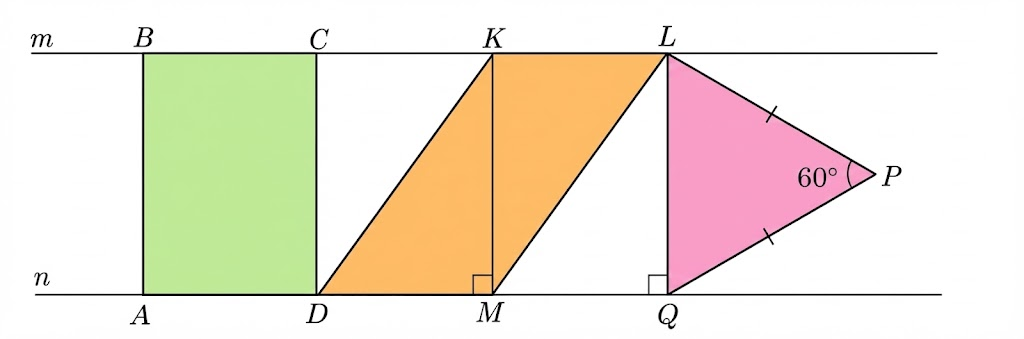
\includegraphics[scale=0.5]{parallel_lines_figures.png}
\end{center}

\nmtnobreak
\nopagebreak\nbvspace{0.3cm}
\matchingLayout{
\matchHead{Фігура}
\matchItem{1}{прямокутник $ABCD$}
\matchItem{2}{паралелограм $DKLM$}
\matchItem{3}{трикутник $LPQ$}
}{
\matchHead{Периметр фігури}
\matchItem{А}{24 \textit{см}}
\matchItem{Б}{32 \textit{см}}
\matchItem{В}{28 \textit{см}}
\matchItem{Г}{36 \textit{см}}
\matchItem{Д}{14 \textit{см}}
}{
\matchingGrid
}
\par\penalty-20\vspace{0.25cm}
\end{samepage}
\endgroup

\instructionBox{Розв'яжіть завдання 19--22. Одержані числові відповіді запишіть у бланку відповідей. Відповідь записуйте лише десятковим дробом, урахувавши положення коми. Знак «мінус» записуйте перед першою цифрою числа.}

\begingroup
% --- макроси з файлів сесій НМТ-2026 (для рисунків) ---
\renewcommand{\headrulewidth}{0.4pt}
\renewcommand{\footrulewidth}{0.4pt}

% --- сумісність зі старою базою (діє, якщо тема не має власного визначення) ---
\providecommand{\trigStyle}[1]{#1}
\providecommand{\answerTableSmall}[5]{%
\begingroup\setlength{\tabcolsep}{2pt}\small\nmtSetCell
\begin{tabular}{|*{5}{>{\centering\arraybackslash}m{\nmtcellw}|}}
\hline
\rule[-0.2cm]{0pt}{0.6cm}\textbf{А} & \textbf{Б} & \textbf{В} & \textbf{Г} & \textbf{Д} \\
\hline
\rule[-0.4cm]{0pt}{0.9cm}#1 & \rule[-0.4cm]{0pt}{0.9cm}#2 & \rule[-0.4cm]{0pt}{0.9cm}#3 & \rule[-0.4cm]{0pt}{0.9cm}#4 & \rule[-0.4cm]{0pt}{0.9cm}#5 \\
\hline
\end{tabular}\endgroup}
\providecommand{\matchingLayout}[3]{%
    \noindent
    \begin{minipage}[t]{0.36\textwidth}\vspace{0pt}\raggedright
        #1
    \end{minipage}%
    \hfill
    \begin{minipage}[t]{0.43\textwidth}\vspace{0pt}\raggedright
        #2
    \end{minipage}%
    \hfill
    \begin{minipage}[t]{0.19\textwidth}
        \vspace{0pt}
        \begin{flushright}
        #3
        \end{flushright}
    \end{minipage}}
\providecommand{\matchingLayoutBottom}[2]{%
    \noindent
    \begin{minipage}[t]{0.48\textwidth}\vspace{0pt}\raggedright
        #1
    \end{minipage}%
    \hfill
    \begin{minipage}[t]{0.48\textwidth}\vspace{0pt}\raggedright
        #2
    \end{minipage}
    \vspace{0.5cm}
    \noindent
    \matchingGrid}
\providecommand{\answerListVertical}[5]{%
    \par\nopagebreak\vspace{0.2cm}
    \begin{itemize}[itemsep=0.4cm, leftmargin=1.5cm, labelsep=0.5cm]
        \item[\textbf{А}] #1
        \item[\textbf{Б}] #2
        \item[\textbf{В}] #3
        \item[\textbf{Г}] #4
        \item[\textbf{Д}] #5
    \end{itemize}
    \vspace{0.2cm}}
\begin{samepage}
\zadtask{Знайдіть площу фігури, обмеженої графіком функції $y = \dfrac{x^3}{8}$, прямими $x = 2$, $x = 4$ та віссю $x$.}
\nmtAnswerBox
\par\penalty-20
\end{samepage}
\endgroup

\begingroup
% --- сумісність зі старою базою (діє, якщо тема не має власного визначення) ---
\providecommand{\trigStyle}[1]{#1}
\providecommand{\answerTableSmall}[5]{%
\begingroup\setlength{\tabcolsep}{2pt}\small\nmtSetCell
\begin{tabular}{|*{5}{>{\centering\arraybackslash}m{\nmtcellw}|}}
\hline
\rule[-0.2cm]{0pt}{0.6cm}\textbf{А} & \textbf{Б} & \textbf{В} & \textbf{Г} & \textbf{Д} \\
\hline
\rule[-0.4cm]{0pt}{0.9cm}#1 & \rule[-0.4cm]{0pt}{0.9cm}#2 & \rule[-0.4cm]{0pt}{0.9cm}#3 & \rule[-0.4cm]{0pt}{0.9cm}#4 & \rule[-0.4cm]{0pt}{0.9cm}#5 \\
\hline
\end{tabular}\endgroup}
\providecommand{\matchingLayout}[3]{%
    \noindent
    \begin{minipage}[t]{0.36\textwidth}\vspace{0pt}\raggedright
        #1
    \end{minipage}%
    \hfill
    \begin{minipage}[t]{0.43\textwidth}\vspace{0pt}\raggedright
        #2
    \end{minipage}%
    \hfill
    \begin{minipage}[t]{0.19\textwidth}
        \vspace{0pt}
        \begin{flushright}
        #3
        \end{flushright}
    \end{minipage}}
\providecommand{\matchingLayoutBottom}[2]{%
    \noindent
    \begin{minipage}[t]{0.48\textwidth}\vspace{0pt}\raggedright
        #1
    \end{minipage}%
    \hfill
    \begin{minipage}[t]{0.48\textwidth}\vspace{0pt}\raggedright
        #2
    \end{minipage}
    \vspace{0.5cm}
    \noindent
    \matchingGrid}
\providecommand{\answerListVertical}[5]{%
    \par\nopagebreak\vspace{0.2cm}
    \begin{itemize}[itemsep=0.4cm, leftmargin=1.5cm, labelsep=0.5cm]
        \item[\textbf{А}] #1
        \item[\textbf{Б}] #2
        \item[\textbf{В}] #3
        \item[\textbf{Г}] #4
        \item[\textbf{Д}] #5
    \end{itemize}
    \vspace{0.2cm}}
\begin{samepage}
\zadtask{Автомобіль двічі заправляли пальним і щоразу по $40$~л. Порівняно з першим заправленням ціна пального, використаного для другого заправлення, була більшою на $2{,}5\,\%$. Усього за ці два заправлення автомобіля пальним було витрачено $4860$~грн. Скільки \textit{гривень} коштував $1$~л пального, використаного під час першого заправлення?}
\nmtAnswerBox
\par\penalty-20
\end{samepage}
\endgroup

\begingroup
% --- макроси, перенесені зі старого файлу теми ---
\providecommand{\matchingLayout}{}\renewcommand{\matchingLayout}[3]{
    \noindent
    \begin{minipage}[t]{0.36\textwidth}\vspace{0pt}\raggedright
       
        #1
    \end{minipage}%
    \hfill
    \begin{minipage}[t]{0.43\textwidth}\vspace{0pt}\raggedright
        
        #2
    \end{minipage}%
    \hfill
    \begin{minipage}[t]{0.19\textwidth}\vspace{0pt}\raggedright
        \vspace{0pt} % Хаки для вирівнювання minipage по верху
        \begin{flushright}
        #3
        \end{flushright}
    \end{minipage}
}

% --- макроси з файлів сесій НМТ-2026 (для рисунків) ---
\renewcommand{\headrulewidth}{0.4pt}
\renewcommand{\footrulewidth}{0.4pt}
\definecolor{hexcol}{RGB}{200,110,60}
\providecommand{\hexthree}{}\renewcommand{\hexthree}[2]{%
    \draw[hexcol, line width=1.1pt]
        ($(#1,#2)+(0:30)$) -- ($(#1,#2)+(60:30)$) -- ($(#1,#2)+(120:30)$) --
        ($(#1,#2)+(180:30)$) -- ($(#1,#2)+(240:30)$) -- ($(#1,#2)+(300:30)$) -- cycle;
}

% --- сумісність зі старою базою (діє, якщо тема не має власного визначення) ---
\providecommand{\trigStyle}[1]{#1}
\providecommand{\answerTableSmall}[5]{%
\begingroup\setlength{\tabcolsep}{2pt}\small\nmtSetCell
\begin{tabular}{|*{5}{>{\centering\arraybackslash}m{\nmtcellw}|}}
\hline
\rule[-0.2cm]{0pt}{0.6cm}\textbf{А} & \textbf{Б} & \textbf{В} & \textbf{Г} & \textbf{Д} \\
\hline
\rule[-0.4cm]{0pt}{0.9cm}#1 & \rule[-0.4cm]{0pt}{0.9cm}#2 & \rule[-0.4cm]{0pt}{0.9cm}#3 & \rule[-0.4cm]{0pt}{0.9cm}#4 & \rule[-0.4cm]{0pt}{0.9cm}#5 \\
\hline
\end{tabular}\endgroup}
\providecommand{\matchingLayout}[3]{%
    \noindent
    \begin{minipage}[t]{0.36\textwidth}\vspace{0pt}\raggedright
        #1
    \end{minipage}%
    \hfill
    \begin{minipage}[t]{0.43\textwidth}\vspace{0pt}\raggedright
        #2
    \end{minipage}%
    \hfill
    \begin{minipage}[t]{0.19\textwidth}
        \vspace{0pt}
        \begin{flushright}
        #3
        \end{flushright}
    \end{minipage}}
\providecommand{\matchingLayoutBottom}[2]{%
    \noindent
    \begin{minipage}[t]{0.48\textwidth}\vspace{0pt}\raggedright
        #1
    \end{minipage}%
    \hfill
    \begin{minipage}[t]{0.48\textwidth}\vspace{0pt}\raggedright
        #2
    \end{minipage}
    \vspace{0.5cm}
    \noindent
    \matchingGrid}
\providecommand{\answerListVertical}[5]{%
    \par\nopagebreak\vspace{0.2cm}
    \begin{itemize}[itemsep=0.4cm, leftmargin=1.5cm, labelsep=0.5cm]
        \item[\textbf{А}] #1
        \item[\textbf{Б}] #2
        \item[\textbf{В}] #3
        \item[\textbf{Г}] #4
        \item[\textbf{Д}] #5
    \end{itemize}
    \vspace{0.2cm}}
\begin{samepage}
\noindent\zadnum \begin{minipage}[t]{0.95\textwidth}
У прямокутній системі координат у просторі задано правильну трикутну призму $ABCA_1B_1C_1$, у якій $A(2; -8; 10)$. Усі ребра призми рівні. Діагоналі грані $BCC_1B_1$ перетинаються в точці $K(12; -2; 7)$. Обчисліть площу бічної поверхні цієї призми.
\end{minipage}
\nmtAnswerBox
\par\penalty-20
\end{samepage}
\endgroup

\begingroup
% --- сумісність зі старою базою (діє, якщо тема не має власного визначення) ---
\providecommand{\trigStyle}[1]{#1}
\providecommand{\answerTableSmall}[5]{%
\begingroup\setlength{\tabcolsep}{2pt}\small\nmtSetCell
\begin{tabular}{|*{5}{>{\centering\arraybackslash}m{\nmtcellw}|}}
\hline
\rule[-0.2cm]{0pt}{0.6cm}\textbf{А} & \textbf{Б} & \textbf{В} & \textbf{Г} & \textbf{Д} \\
\hline
\rule[-0.4cm]{0pt}{0.9cm}#1 & \rule[-0.4cm]{0pt}{0.9cm}#2 & \rule[-0.4cm]{0pt}{0.9cm}#3 & \rule[-0.4cm]{0pt}{0.9cm}#4 & \rule[-0.4cm]{0pt}{0.9cm}#5 \\
\hline
\end{tabular}\endgroup}
\providecommand{\matchingLayout}[3]{%
    \noindent
    \begin{minipage}[t]{0.36\textwidth}\vspace{0pt}\raggedright
        #1
    \end{minipage}%
    \hfill
    \begin{minipage}[t]{0.43\textwidth}\vspace{0pt}\raggedright
        #2
    \end{minipage}%
    \hfill
    \begin{minipage}[t]{0.19\textwidth}
        \vspace{0pt}
        \begin{flushright}
        #3
        \end{flushright}
    \end{minipage}}
\providecommand{\matchingLayoutBottom}[2]{%
    \noindent
    \begin{minipage}[t]{0.48\textwidth}\vspace{0pt}\raggedright
        #1
    \end{minipage}%
    \hfill
    \begin{minipage}[t]{0.48\textwidth}\vspace{0pt}\raggedright
        #2
    \end{minipage}
    \vspace{0.5cm}
    \noindent
    \matchingGrid}
\providecommand{\answerListVertical}[5]{%
    \par\nopagebreak\vspace{0.2cm}
    \begin{itemize}[itemsep=0.4cm, leftmargin=1.5cm, labelsep=0.5cm]
        \item[\textbf{А}] #1
        \item[\textbf{Б}] #2
        \item[\textbf{В}] #3
        \item[\textbf{Г}] #4
        \item[\textbf{Д}] #5
    \end{itemize}
    \vspace{0.2cm}}
\begin{samepage}
\noindent\zadnum Визначте кількість усіх цілих значень $a$ з проміжку $[-11; 11]$, за кожного з яких рівняння $\sqrt{2x - a + 4} \cdot (\log_2 x - 2) = 0$ має два різних корені.

\nmtnobreak
\nopagebreak\nbvspace{0.3cm}
\nmtAnswerBox
\par\penalty-20
\end{samepage}
\endgroup

\clearpage
\sectionTitle{Відповіді}

\begin{center}\small\renewcommand{\arraystretch}{1.25}
\begin{tabular}{|c|c|p{0.62\textwidth}|}\hline
\textbf{№} & \textbf{Відповідь} & \textbf{Джерело завдання} \\ \hline
1 & Г & НМТ 2025, сесія 06.06.2025, № 9 \\ \hline
2 & Б & НМТ 2026, сесія 05.06.2026, № 2 \\ \hline
3 & Д & НМТ 2025, сесія 17.06.2025, № 3 \\ \hline
4 & В & НМТ 2024, сесія 21.06.2024, № 4 \\ \hline
5 & Д & НМТ 2025 \\ \hline
6 & А & НМТ 2023, сесія 14.06.2023, 2 зміна, № 6 \\ \hline
7 & Б & НМТ 2023, сесія 19.06.2023, 2 зміна, № 5 \\ \hline
8 & Д & НМТ 2026, сесія 02.06.2026, № 8 \\ \hline
9 & В & НМТ 2026, сесія 17.06.2026, № 9 \\ \hline
10 & В & НМТ 2025, сесія 09.06.2025, № 6 \\ \hline
11 & А & НМТ 2024, сесія 05.06.2024, № 1 \\ \hline
12 & А & НМТ 2025, сесія 05.06.2025, № 10 \\ \hline
13 & Д & НМТ 2024 \\ \hline
14 & Г & НМТ 2023, сесія 20.06.2023, 2 зміна, № 14 \\ \hline
15 & Б & НМТ 2025, сесія 13.06.2025, № 15 \\ \hline
16 & 1~--~А, 2~--~Д, 3~--~Г & НМТ 2025, сесія 31.05.2025, № 18 \\ \hline
17 & 1~--~А, 2~--~Г, 3~--~Б & НМТ 2025, сесія 09.06.2025, № 17 \\ \hline
18 & 1~--~В, 2~--~Б, 3~--~А & НМТ 2025, сесія 11.06.2025, № 18 \\ \hline
19 & $7{,}5$ & НМТ 2026, сесія 19.06.2026, № 19 \\ \hline
20 & $60$ & НМТ 2026, сесія 17.06.2026, № 20 \\ \hline
21 & $435$ & НМТ 2024, сесія 25.05.2024, № 21 \\ \hline
22 & $7$ & НМТ 2024, сесія 18.05.2024, № 22 \\ \hline
\end{tabular}\end{center}

\noindent{\small\color{gray!80!black}Оцінювання: завдання 1--15 -- по 1 балу; 16--18 -- по 1 балу за кожну правильно встановлену відповідність (до 3 балів); 19--22 -- по 2 бали. Разом 32 бали.}

\end{document}
